%!TEX root = edance.tex
%%%%%%%%%%%%%%%%
%   CHAPTER 3  %
%%%%%%%%%%%%%%%%
\chapter{Introduction to Semiconductors}
\graphicspath{{./figs_semi/}}
%%%%%%%%%%%%%%%%%%%%%%%%%%%%%%%%%%%%%%%%%%%%%%%%%%%%%%%%%%%%%%%%%%%%%%%%%%%%%%%%%%%%%%%%
%%%%%%%%%%%%%%%%%%%%%%%%%%%%%%%%%%%%%%%%%%%%%%%%%%%%%%%%%%%%%%%%%%%%%%%%%%%%%%%%%%%%%%%%
%                                   SECTION 3.1                                        %
%%%%%%%%%%%%%%%%%%%%%%%%%%%%%%%%%%%%%%%%%%%%%%%%%%%%%%%%%%%%%%%%%%%%%%%%%%%%%%%%%%%%%%%%
%%%%%%%%%%%%%%%%%%%%%%%%%%%%%%%%%%%%%%%%%%%%%%%%%%%%%%%%%%%%%%%%%%%%%%%%%%%%%%%%%%%%%%%%
\section{Chapter Preview}
In this chapter we'll build models for conductors and semiconductors, starting with the simplest model of all, an ideal metal with a "gas" of electrons swarming about and study conduction in this ideal system.  Surprisingly, we'll find that many properties of real conductors are captured with this model.  Next, we'll delve into semiconductors and learn why the model breaks down.  We'll briefly look a the structure of semiconductors and then develop a simple bond model that can account for free carriers, especially when a material is "doped", or when impurities are added to a solid to modulate its conductivity.  With this model in hand, we'll discuss drift and diffusion currents.  Drift currents are already familiar conduction of electrons in response to a field, or Ohm's Law, whereas diffusion current is due to concentration gradients, which play an important role in devices like diodes. 
%%%%%%%%%%%%%%%%%%%%%%%%%%%%%%%%%%%%%%%%%%%%%%%%%%%%%%%%%%%%%%%%%%%%%%%%%%%%%%%%%%%%%%%%
%%%%%%%%%%%%%%%%%%%%%%%%%%%%%%%%%%%%%%%%%%%%%%%%%%%%%%%%%%%%%%%%%%%%%%%%%%%%%%%%%%%%%%%%
%                                   SECTION 3.2                                        %
%%%%%%%%%%%%%%%%%%%%%%%%%%%%%%%%%%%%%%%%%%%%%%%%%%%%%%%%%%%%%%%%%%%%%%%%%%%%%%%%%%%%%%%%
%%%%%%%%%%%%%%%%%%%%%%%%%%%%%%%%%%%%%%%%%%%%%%%%%%%%%%%%%%%%%%%%%%%%%%%%%%%%%%%%%%%%%%%%
\section{Conduction in an Ideal Metal ``Gas''}
%%%%%%%%%%%%%%%%%%%%%%%%%%%%%%%%%%%%%%%%%%%%
%             SUBSECTION 3.2.1             %
%%%%%%%%%%%%%%%%%%%%%%%%%%%%%%%%%%%%%%%%%%%%
\subsection{Ohm’s Law}
One of the first things we learn in electrical engineering and physics is that  $V = I \times R$.
Is this trivial? Maybe what’s really going on is the following:
    \begin{equation}
        V = f(I) = f(0) + f'(0)I + f''(0){I^2}/2 + ... \approx f'(0)I
    \end{equation}
In the above Taylor expansion, if the voltage is zero for zero current, and the current is small, then this is generally valid for a reasonably smooth function.   The range of validity (radius of convergence) is the important question. It turns out to be VERY large!
%%%%%%%%%%%%%%%%%%%%%%%%%%%%%%%%%%%%%%%%%%%%
%             SUBSECTION 3.2.2             %
%%%%%%%%%%%%%%%%%%%%%%%%%%%%%%%%%%%%%%%%%%%%
\subsection{Ohm’s Law Revisited}
 In Physics we learned:  $J = \sigma \,E$  Is this also trivial? Well, it’s the same as Ohm’s law, so the questions are related. For a rectangular solid:
\begin{equation}
        J = \frac{I}{A} = \sigma \,\frac{V}{L} \end{equation}\begin{equation}  V = \frac{L}{{\sigma \,A}}I = R\,I
\end{equation}
Isn’t it strange that current (velocity) is proportional to Force?  Where does conductivity come from?
%%%%%%%%%%%%%%%%%%%%%%%%%%%%%%%%%%%%%%%%%%%%
%             SUBSECTION 3.2.3             %
%%%%%%%%%%%%%%%%%%%%%%%%%%%%%%%%%%%%%%%%%%%%
\subsection{Conductivity of a Gas}
Electrical conduction is due to the motion of positive and negative charges.   For example, for  water with pH=7, the concentration of hydrogen H+ ions (and OH-) is:
\begin{equation}
{10^{ - 7}}{\rm{mole/L}} = {\rm{1}}{{\rm{0}}^{{\rm{ - 10}}}}{\rm{mole/c}}{{\rm{m}}^{\rm{3}}}
= {\rm{1}}{{\rm{0}}^{{\rm{ - 10}}}} \times 6.02 \times {10^{23}}{\rm{c}}{{\rm{m}}^{ - 3}}
= 6 \times {10^{13}}{\rm{c}}{{\rm{m}}^{ - 3}}
\end{equation}
Typically, the concentration of charged carriers is much smaller than the concentration of neutral molecules.   The motion of the charged carriers (electrons, ions, molecules) gives rise to electrical conduction.
%%%%%%%%%%%%%%%%%%%%%%%%%%%%%%%%%%%%%%%%%%%%
%              SUB-SUBSECTION              %
%%%%%%%%%%%%%%%%%%%%%%%%%%%%%%%%%%%%%%%%%%%%
\subsubsection{Collisions in Gas}
At a temperate $T$, each charged carrier will move in a random direction and velocity until it encounters a neutral molecule or another charged carrier.  Since the concentration of charged carriers is much less than molecules, it will most likely encounter a molecule. For a gas, the molecules are widely separated ($\sim 10$ molecular diameters).  After colliding with the molecule, there is some energy exchange and the charge carrier will come out with a new velocity and new direction.
%%%%%%%%%%%%%%%%%%%%%%%%%%%%%%%%%%%%%%%%%%%%
%              SUB-SUBSECTION              %
%%%%%%%%%%%%%%%%%%%%%%%%%%%%%%%%%%%%%%%%%%%%
\subsubsection{Memory Loss in Collisions}
 Schematically our model thus far is shown in Fig.~\ref{fig:slide8}.   The key point is the initial velocity and direction is lost (randomized) after a few collisions.
%%%%%%%%%%%%%%%%%%%%%%%%%%%%%%%%%%%%%%%%%%%%
%                 FIGURE                   %
%%%%%%%%%%%%%%%%%%%%%%%%%%%%%%%%%%%%%%%%%%%%
\begin{figure}
\centering
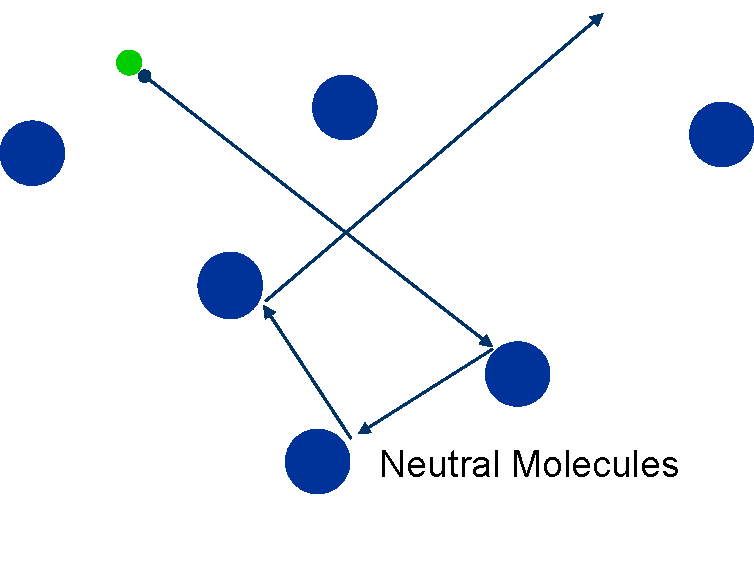
\includegraphics[width=.4\columnwidth]{slide8}
\caption{Simple model for a charged particle like an electron moving in a random array of atoms or molecules.  We assume the particle moves freely until it encounters an atom or molecule, causing it to scatter off in a new direction with a new speed.}
\label{fig:slide8}
\end{figure}
%%%%%%%%%%%%%%%%%%%%%%%%%%%%%%%%%%%%%%%%%%%%
%              SUB-SUBSECTION              %
%%%%%%%%%%%%%%%%%%%%%%%%%%%%%%%%%%%%%%%%%%%%
\subsubsection{Application of Field}
When we apply an electric field, during each “free flight”, the carriers will gain a momentum of $ {\bf{E}}qt $.  Therefore, after $t$ seconds, the momentum is given by:
\begin{equation}
        M{\bf{u}} + {\bf{E}}qt
\end{equation}
If we take the average momentum of all particles at any given time, we have:
\begin{equation}
        M{\bf{\bar u}} = \frac{1}{N}\sum\limits_j {\left( {M{{\bf{u}}_j} + {\bf{E}}q{t_j}} \right)}
\end{equation}
In this equation, $ N $ is the number of carriers (of charge), $ M \bf{u}_j $ is the initial momentum before collision, and $\bf{E}q{t_j}$ is the momentum gained from the field in the time $t_j$ from the last collision.
%%%%%%%%%%%%%%%%%%%%%%%%%%%%%%%%%%%%%%%%%%%%
%              SUB-SUBSECTION              %
%%%%%%%%%%%%%%%%%%%%%%%%%%%%%%%%%%%%%%%%%%%%
\subsubsection{Random Things Sum to Zero!}
When we sum over all the random velocities of the particles, we are averaging over a large number of random variables with zero mean, the average is zero:
\begin{equation}
        M{\bf{\bar u}} = \frac{1}{N}\sum\limits_j {\left( {M{{\bf{u}}_j} + {\bf{E}}q{t_j}} \right)}
\end{equation}
which allows us to ignore the first sum, leading to
\begin{equation}
        M{\bf{\bar u}} = \frac{1}{N}\sum\limits_j {{\bf{E}}q{t_j}}  = {\bf{E}}q\tau
\end{equation}
So the current is given by
\begin{equation} {\bf{J}} = Nq{\bf{\bar u}} = Nq\left( {\frac{{{\bf{E}}q\tau }}{M}} \right) = N{q^2}\frac{\tau }{M}{\bf{E}} = \sigma \,{\bf{E}}
\end{equation}
%%%%%%%%%%%%%%%%%%%%%%%%%%%%%%%%%%%%%%%%%%%%
%             SUBSECTION 3.2.4             %
%%%%%%%%%%%%%%%%%%%%%%%%%%%%%%%%%%%%%%%%%%%%
\subsection{Mobility}
From the previous derivation, we see that the average momentum gain from the field is given by:
\begin{equation}
        {\bf{J}} = {{\bf{J}}^ + } - {{\bf{J}}^ - } = e\left( {\frac{{{N^ + }e{\tau ^ + }}}{{{M^ + }}} - \frac{{ - {N^ - }e{\tau ^ - }}}{{{M^ - }}}} \right){\bf{E}}
\end{equation}
In many situations we’d like to find the average speed gained from the field, which is defined as  the mobility ($\mu$):
\begin{equation}
        \mu  = {e^2}\left( {\frac{{{N^ + }{\tau ^ + }}}{{{M^ + }}} + \frac{{{N^ - }{\tau ^ - }}}{{{M^ - }}}} \right)  
\end{equation}
So we see that even though we apply an electric field, applying a force to electrons, they don't accelerate like free electrons.  Instead they gain only a fixed amount of momentum, not linearly increasing in time as predicted for free electrons.

A good analogy is the following.  Imagine driving a car on a busy freeway, a stop-and-go situation.  Every time you have the opportunity to move, you accelerate a certain amount of time but very soon the car in front of you stops, forcing you to hit the breaks.  So even though you're accelerating, or trying to accelerate forward, you're actually just able to gain momentum for brief periods of time in between the stops.  In a similar fashion, when electrons or other charges accelerate under the application of a field, they only do so for a short period of time, in between collisions, and so they can only gain a bit of  momentum on average before they are forced to stop and try again, rather than continuously gaining momentum from the field such as in free space.
%%%%%%%%%%%%%%%%%%%%%%%%%%%%%%%%%%%%%%%%%%%%
%              SUB-SUBSECTION              %
%%%%%%%%%%%%%%%%%%%%%%%%%%%%%%%%%%%%%%%%%%%%
\subsubsection{Negative and Positive Carriers}
Since current is contributed by positive and negative charge carriers:
\begin{equation}
        {\bf{J}} = {{\bf{J}}^ + } - {{\bf{J}}^ - } = e\left( {\frac{{{N^ + }e{\tau ^ + }}}{{{M^ + }}} - \frac{{ - {N^ - }e{\tau ^ - }}}{{{M^ - }}}} \right){\bf{E}}
\end{equation}
Or in terms of mobility:
\begin{equation}
        \sigma  = {e^2}\left( {\frac{{{N^ + }{\tau ^ + }}}{{{M^ + }}} + \frac{{{N^ - }{\tau ^ - }}}{{{M^ - }}}} \right)
\end{equation}
%%%%%%%%%%%%%%%%%%%%%%%%%%%%%%%%%%%%%%%%%%%%
%             SUBSECTION 3.2.5             %
%%%%%%%%%%%%%%%%%%%%%%%%%%%%%%%%%%%%%%%%%%%%
\subsection{Conduction in Metals}
Can we apply this simple "gas" model to a conductor?  The  high conductivity of metals is due to large concentration of free electrons.   These electrons are not attached to the solid but are free to move about the solid.  In other words, we have an "electron gas".   In metal sodium, for example,  each atom contributes a free electron: 
\[
        N = 2.5 \times {10^{22}}{\rm{atoms/c}}{{\rm{m}}^{\rm{3}}}
\]
From the measured value of conductivity (easy to make in the lab), we can back calculate the mean free time:
\begin{equation}\tau  = \frac{{\sigma \,m}}{{N{e^2}}} = \frac{{\left( {1.9 \times {{10}^{17}}} \right)\,\left( {9 \times {{10}^{ - 28}}} \right)}}{{\left( {2.5 \times {{10}^{22}}} \right)\,\left( {23 \times {{10}^{ - 20}}} \right)}} = 3 \times {10^{ - 14}}\sec
\end{equation}
%%%%%%%%%%%%%%%%%%%%%%%%%%%%%%%%%%%%%%%%%%%%
%              SUB-SUBSECTION              %
%%%%%%%%%%%%%%%%%%%%%%%%%%%%%%%%%%%%%%%%%%%%
\subsubsection{A Deep Puzzle}
This value of mean free time is surprisingly long.  The mean velocity for an electron at room temperature is about: 
\begin{equation}
        \frac{{m{v^2}}}{2} = \frac{3}{2}kT  v = 3 \times {10^7}{\rm{cm}}/\sec
\end{equation}
At this speed, the electron travels a distance of $v\tau  = 3 \times {10^{ - 7}}{\rm{cm}}$.  The molecular spacing between adjacent ions is only $3.8 \times {10^{ - 8}}{\rm{cm}}$.  Why is it that the electron is on average zooming by 10 positively charged ions?
%%%%%%%%%%%%%%%%%%%%%%%%%%%%%%%%%%%%%%%%%%%%
%             SUBSECTION 3.2.6             %
%%%%%%%%%%%%%%%%%%%%%%%%%%%%%%%%%%%%%%%%%%%%
\subsection{Wave Nature of Electron}
%%%%%%%%%%%%%%%%%%%%%%%%%%%%%%%%%%%%%%%%%%%%
%                 FIGURE                   %
%%%%%%%%%%%%%%%%%%%%%%%%%%%%%%%%%%%%%%%%%%%%
\begin{figure}
\centering
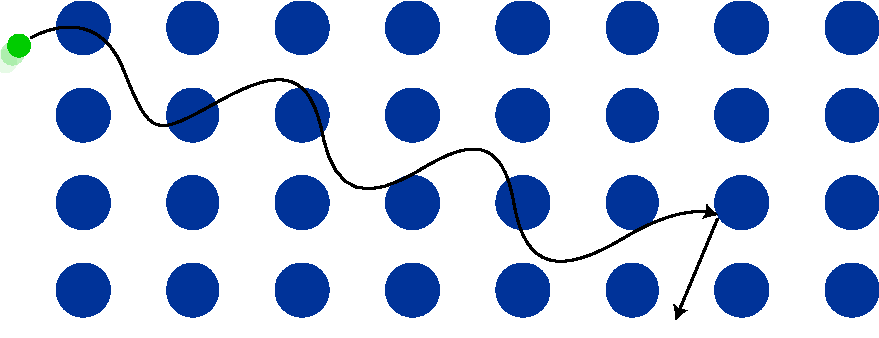
\includegraphics[width=.75\columnwidth]{crystal_blochwave}
\caption{Measurements show that the average distance electrons move in a crystal is much larger than the inter-atomic distance, indicating that the electrons somehow move through the nuclei unperturbed.  In fact, a free electron in a periodic arrangement of atoms can move freely around the crystal as a "free particle" with an \emph{effective mass} that takes into account the potential of the nuclei in the crystal.  In other words, the electron does not scatter simply because it encounters an atom.}
\label{fig:slide15}
\end{figure}

 The free carrier can penetrate right through positively charged host atoms, as shown schematically in Fig.~\ref{fig:slide15}!  Quantum mechanics explains this!  For a periodic arrangement of potential functions, the electron does not scatter. The influence of the crystal is that it will travel freely with an effective mass different from the rest mass or free electron mass.   So why does it scatter at all?
%%%%%%%%%%%%%%%%%%%%%%%%%%%%%%%%%%%%%%%%%%%%
%             SUBSECTION 3.2.7             %
%%%%%%%%%%%%%%%%%%%%%%%%%%%%%%%%%%%%%%%%%%%%
\subsection{Scattering in Metals}
At temperature $T$, the atoms are in random motions in the host atoms (see Fig.~\ref{fig:slide16}a), and so the potential function experienced by charged carriers is not periodic, but quasi-periodic. 
%%%%%%%%%%%%%%%%%%%%%%%%%%%%%%%%%%%%%%%%%%%%
%                 FIGURE                   %
%%%%%%%%%%%%%%%%%%%%%%%%%%%%%%%%%%%%%%%%%%%%
\begin{figure}
\centering
\begin{tabular}{ccc}
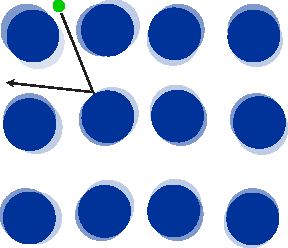
\includegraphics[width=.3\columnwidth]{lattice_vibrate} &
\hspace{.15\columnwidth} &
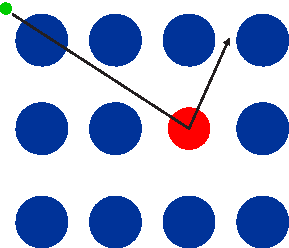
\includegraphics[width=.3\columnwidth]{lattice_impurity}\\
(a) & & (b)\\
\end{tabular}
\caption{(a) The random thermal motion of atoms in a crystal (\emph{lattice vibrations}) disturbs the periodicity of the array and results in scattering of free carriers.  (b) The presence of an impurity atom (shown in red) also disturbs the periodicity of the array and results in scattering.}
\label{fig:slide16}
\end{figure}
%%%%%%%%%%%%%%%%%%%%%%%%%%%%%%%%%%%%%%%%%%%%
Even at extremely low temperatures, the presence of an impurity upsets the periodicity, as shown in Fig.~\ref{fig:slide16}b.  These two mechanisms, vibrations in the crystal (phonons in the parlance of solid-state physics) and impurities are the source of scattering, and thus resistance, in metals.
%%%%%%%%%%%%%%%%%%%%%%%%%%%%%%%%%%%%%%%%%%%%
%             SUBSECTION 3.2.8             %
%%%%%%%%%%%%%%%%%%%%%%%%%%%%%%%%%%%%%%%%%%%%
\subsection{Summary of Conduction}
Using our ideal gas model for conductors, we have the following result:
\begin{equation}
        \sigma  = {e^2}\left( {\frac{{{N^ + }{\tau ^ + }}}{{{M^ + }}} + \frac{{{N^ - }{\tau ^ - }}}{{{M^ - }}}} \right)
\end{equation}
The conductivity is determined by the density of free charge carriers (both positive and negative), the charge of carrier (usually just \textit{e}), the effective mass of carrier (different inside solid), and the mean relaxation time (time for memory loss … usually the time between collisions).   This is turn is determined by several mechanisms, e.g. scattering by impurities and scattering due to vibrations in crystal.
%%%%%%%%%%%%%%%%%%%%%%%%%%%%%%%%%%%%%%%%%%%%%%%%%%%%%%%%%%%%%%%%%%%%%%%%%%%%%%%%%%%%%%%%
%%%%%%%%%%%%%%%%%%%%%%%%%%%%%%%%%%%%%%%%%%%%%%%%%%%%%%%%%%%%%%%%%%%%%%%%%%%%%%%%%%%%%%%%
%                                   SECTION 3.3                                        %
%%%%%%%%%%%%%%%%%%%%%%%%%%%%%%%%%%%%%%%%%%%%%%%%%%%%%%%%%%%%%%%%%%%%%%%%%%%%%%%%%%%%%%%%
%%%%%%%%%%%%%%%%%%%%%%%%%%%%%%%%%%%%%%%%%%%%%%%%%%%%%%%%%%%%%%%%%%%%%%%%%%%%%%%%%%%%%%%%
\section{Introduction to Semiconductors}
%%%%%%%%%%%%%%%%%%%%%%%%%%%%%%%%%%%%%%%%%%%%
%             SUBSECTION 3.3.1             %
%%%%%%%%%%%%%%%%%%%%%%%%%%%%%%%%%%%%%%%%%%%%
\subsection{Resistivity for a Few Materials}
Let's take a careful look at the conductivity for a few different materials:
\vspace{.5cm}
\begin{minipage}[c]{.55\textwidth}
\begin{itemize}
\item  Pure copper, 273K \hfill 6.4×10$^{7}$ S/m
\item Pure copper, 373K \hfill 4.46×10$^{6}$ S/m
\item Pure germanium, 273K \hfill 0.5  S/m
\item Pure germanium, 500K \hfill 833 S/m
\item Pure water, 291K \hfill 4×10$^{-6}$ S/m
\item Seawater\hfill 4 S/m
\end{itemize} 
\end{minipage}
\vspace{.5cm}
This list is very interesting in several ways.  First of all we see that copper, a good conductor, is in fact a fantastic conductor, with a conductivity several orders of magnitude larger than a material like germanium.  Germanium is a "semi" conductor, or just semiconductor, for obvious reasons.  It conducts, but very poorly.  Also, whereas temperature has a relatively minor impact on the conductivity of copper, decreasing by about 30\% when the temperature is increased by $100^\circ$, germanium seems to be much more sensitive.  The trends are also opposite as germanium is becoming more conductive, by orders of magnitude, with increasing temperature !  Why?

Finally, we have pure water, which is an insulator, because in pure water there are essentially no free charges.  But sea water (and human tissue) is moderately conductive, but it doesn't have the same sensitivity to temperate as a semiconductor.

We have several mysteries on hand !
What gives rise to this enormous range?
Why are some materials semi-conductive?
Why the strong temperature dependence for semiconductors?
%%%%%%%%%%%%%%%%%%%%%%%%%%%%%%%%%%%%%%%%%%%%
%              SUB-SUBSECTION              %
%%%%%%%%%%%%%%%%%%%%%%%%%%%%%%%%%%%%%%%%%%%%
\subsubsection{Periodic Table of Elements}
%%%%%%%%%%%%%%%%%%%%%%%%%%%%%%%%%%%%%%%%%%%%
%                 FIGURE                   %
%%%%%%%%%%%%%%%%%%%%%%%%%%%%%%%%%%%%%%%%%%%%
\begin{figure}
\centering
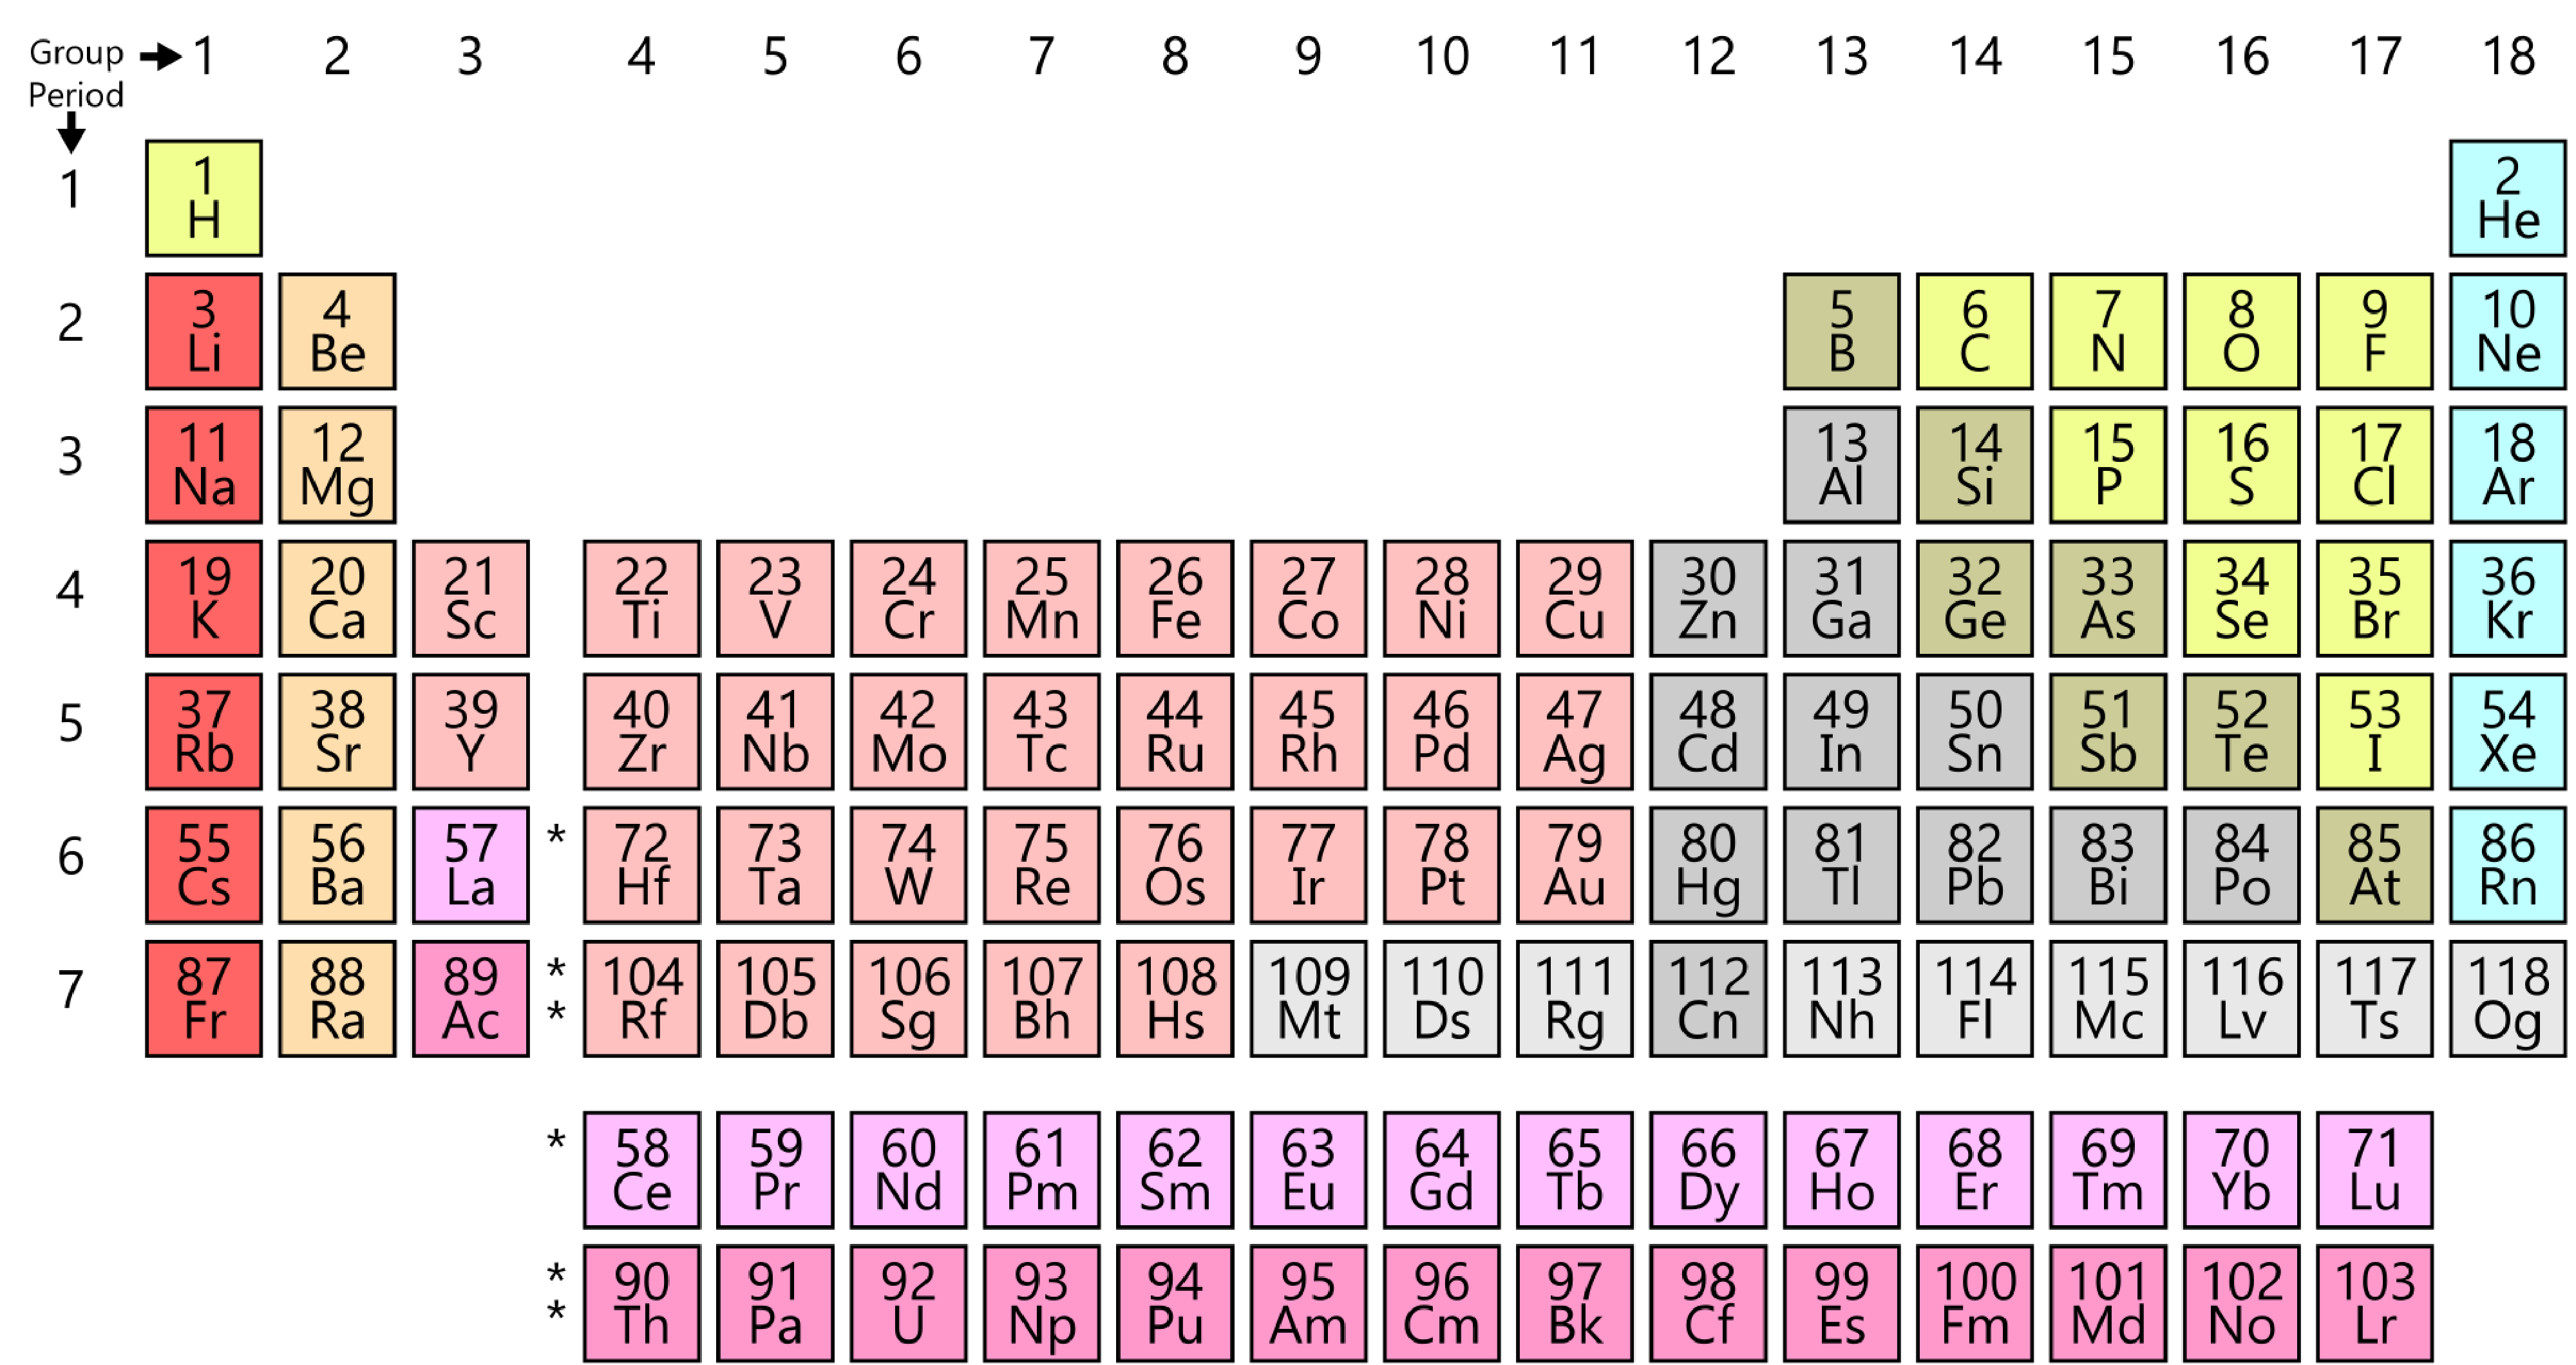
\includegraphics[width=\columnwidth]{periodic_table}
\caption{Periodic table of elements.  Note that many semiconductors are either group 4 elements or combinations of group 3 and 5 elements. Credit:  By Offnfopt - Own work, Public Domain, \url{https://commons.wikimedia.org/w/index.php?curid=62296883}}
\label{fig:periodic_table}
\end{figure}
%%%%%%%%%%%%%%%%%%%%%%%%%%%%%%%%%%%%%%%%%%%%
Have a look at the periodic table reproduced here in Fig.~\ref{fig:periodic_table}.  You may recognize that many semiconductors are either Group III, IV, or V elements.  What is special about Group III, IV, and V elements?  Recall that the number of outer shell electrons in atoms is related to its group number.  Noble gases are unique in that they have complete shells and this is in fact why they are so stable.  Group IV elements in particular have four electrons in their outer shell.  This is why when they are grouped together, they bond and share electrons, four electrons on average.
%%%%%%%%%%%%%%%%%%%%%%%%%%%%%%%%%%%%%%%%%%%%
%             SUBSECTION 3.3.2             %
%%%%%%%%%%%%%%%%%%%%%%%%%%%%%%%%%%%%%%%%%%%%
\subsection{Electronic Properties of Silicon}
We'll focus on silicon, but a lot of what we have to say applies to most semiconductors.  Silicon is the most commonly used semiconductor, so it's the most relevant example.  From chemistry, we know that silicon is in Group IV element, like carbon.  It has a total of 14 electrons, arranged into the following orbital structure shown in Fig.~\ref{fig:slide20}:
\begin{itemize}
\item   Atom electronic structure: 1s$^2$2s$^2$2p$^6$3s$^2$3p$^2$
\item   Crystal electronic structure: 1s$^2$2s$^2$2p$^6$3(sp)$^4$
\item   Diamond lattice, with 0.235 nm bond length
\end{itemize}
 
Notice that the s and p orbitals combine when the silicon atoms combine into a hybridized state.  This deserves a bit of explanation.  When silicon atoms are far apart, the electrons occupy the usual orbital states you're familiar with from chemistry.  The last two electrons are in the p orbital, which can hold a total of 6.  But when the atoms are brought into close proximity, the outer shell valence electrons feel the influence of two nuclei, and therefore it's logical to assume that the electrons should spend more time in between the nuclei, essentially forming covalent bonds.  If the Pauli exclusion principle didn't apply, then all the electrons would occupy the p orbitals in between the silicon atoms, leaving some empty and some more than full !  But alas only 2 electrons per orbital (with opposite spin).

On the other hand, the geometry of the p orbitals shown in Fig.~\ref{fig:slide20} would be ideal if silicon could bond to six neighbors, , but this doesn't happen because there would be too many valence electrons since each atom already has 2 3p electrons, since silicon only needs 4 additional electrons to form a complete shell.  On the other hand, the hybridized 3(sp)$^4$ state (linear combination of s and p orbitals) contains four electrons and can bond with four neighbors as shown.  This scenario is how silicon atoms combine to form a crystal, with the geometry more complicated than a simple cube  arising from these bond angles.

Also, silicon is a very poor conductor at room temperature. Why?
%%%%%%%%%%%%%%%%%%%%%%%%%%%%%%%%%%%%%%%%%%%%
%                 FIGURE                   %
%%%%%%%%%%%%%%%%%%%%%%%%%%%%%%%%%%%%%%%%%%%%
\begin{figure}
\centering
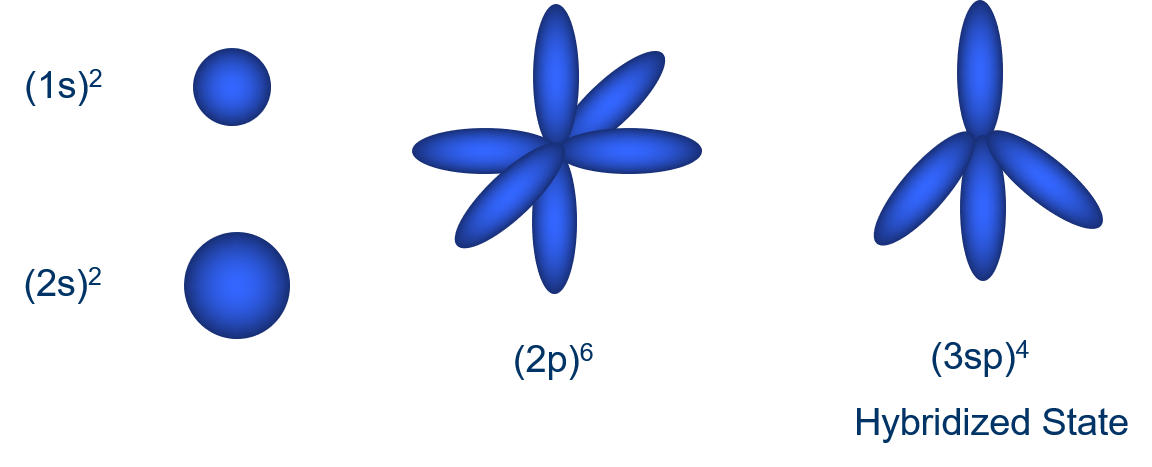
\includegraphics[width=.75\columnwidth]{slide20}
\caption{The s and p orbitals of the isolated silicon atoms and the 3sp hybridized state consisting of a linear combination of p and s orbitals.  When silicon atoms form covalent bonds, the hybridized state is preferred and results in a lower energy configuration.}
\label{fig:slide20}
\end{figure}
%%%%%%%%%%%%%%%%%%%%%%%%%%%%%%%%%%%%%%%%%%%%
%              SUB-SUBSECTION              %
%%%%%%%%%%%%%%%%%%%%%%%%%%%%%%%%%%%%%%%%%%%%
\subsubsection{Si Diamond Structure}
%%%%%%%%%%%%%%%%%%%%%%%%%%%%%%%%%%%%%%%%%%%%
%                 FIGURE                   %
%%%%%%%%%%%%%%%%%%%%%%%%%%%%%%%%%%%%%%%%%%%%
\begin{figure}
\centering
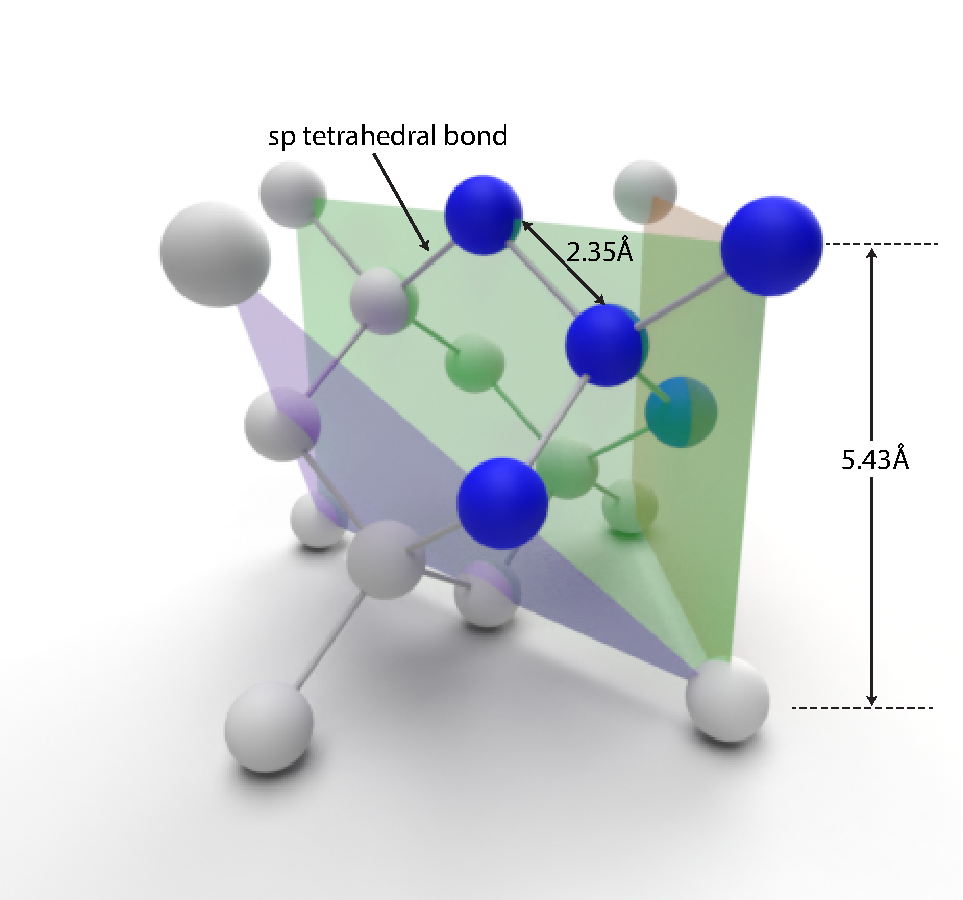
\includegraphics[width=.75\columnwidth]{silicon_crysal_label.pdf}
\caption{The crystal structure of silicon.  All atoms are silicon, and have covalent bonds with their four neighbors.  The colored atoms in this 3D model represent a unit cell that is repeated across the crystal.  The symmetry planes are also highlighted.  A 3D model can be viewed and manipulated online \url{https://sketchfab.com/3d-models/silicon-crystal-lattice-73e292f32ffe4ca490e166faeba317e7}.} \label{fig:silicon_crysal}
\end{figure}
%%%%%%%%%%%%%%%%%%%%%%%%%%%%%%%%%%%%%%%%%%%%
Silicon atoms arrange in a nice crystal structure known as the diamond structure shown in Fig.~\ref{fig:silicon_crysal}.  In this figure, spheres represent silicon atoms with one particular unit cell highlighted.  The planes in the figure correspond to the symmetry planes of the crystal.  Usually the crystal is cut along one of these symmetry planes.

Notice that each silicon atom bonds to four neighbors using a covalent (shared electron) bond.  In a covalent bonds, the electrons are shared among a group of host atoms, giving up their identity and loyalty to a fixed atom as they are shared among a group of nuclei, forming a more stable overall structure than if they remained in their lone atomic orbitals.  The inner core electrons, on the other hand, are bound to the host nucleus and don't participate in conduction (the interest of this chapter) unless very energetic particles such as x-rays are incident on the crystal. 
%%%%%%%%%%%%%%%%%%%%%%%%%%%%%%%%%%%%%%%%%%%%
%             SUBSECTION 3.3.3             %
%%%%%%%%%%%%%%%%%%%%%%%%%%%%%%%%%%%%%%%%%%%%
\subsection{States of an Atom}
%%%%%%%%%%%%%%%%%%%%%%%%%%%%%%%%%%%%%%%%%%%%
%                 FIGURE                   %
%%%%%%%%%%%%%%%%%%%%%%%%%%%%%%%%%%%%%%%%%%%%
\begin{figure}
\centering
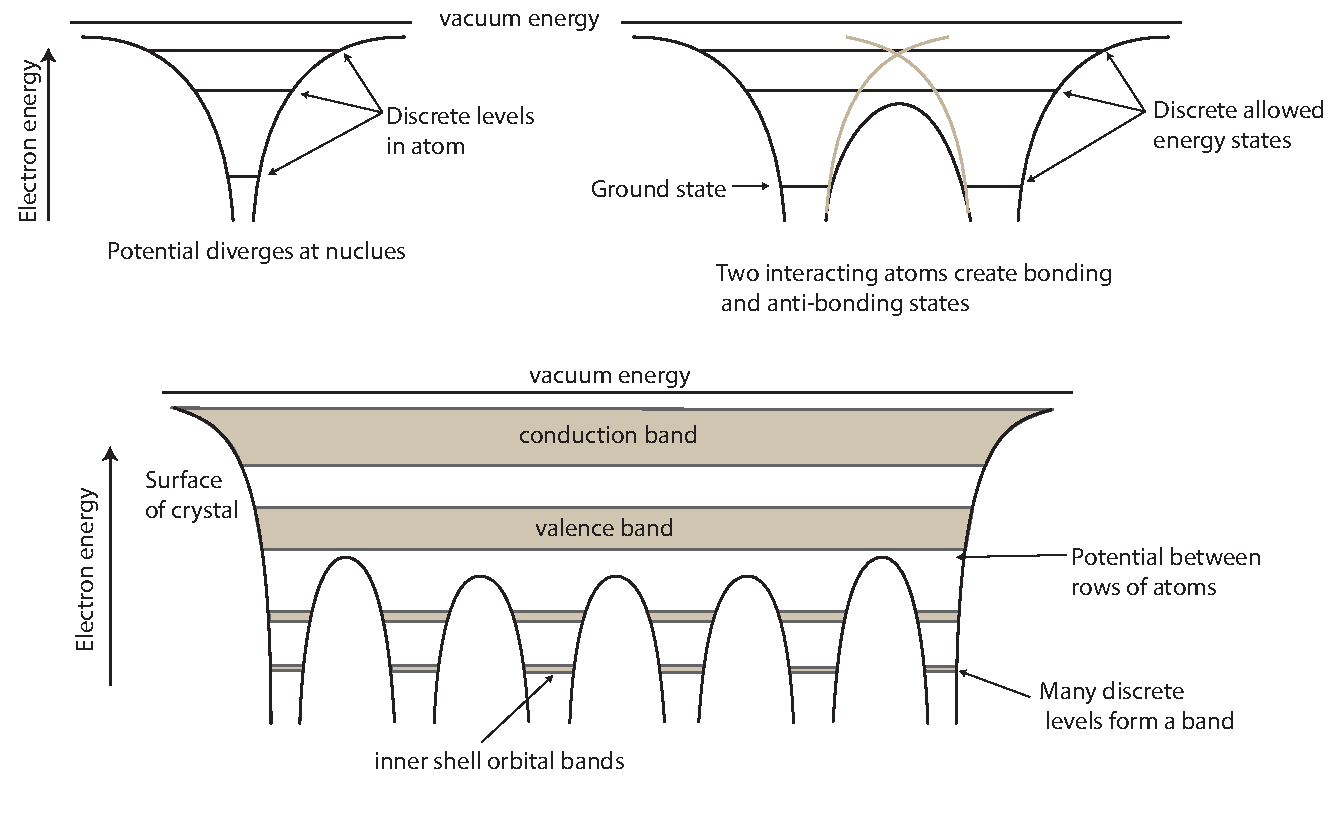
\includegraphics[width=1\columnwidth]{banddiagram_atoms.pdf}
\caption{On the top left we have the discrete energy levels for isolated atoms.  Electrons are only found to have discrete energy level with forbidden energy levels in between allowed states.    We now imagine bringing two atoms closer and closer together as shown on the top right.  Due to their interaction, the energy levels split into bonding and non-bonding states.  When many atoms are involved (bottom), these splittings become very fine forming an almost continuous band of allowed energy levels.  The top two bands called the conduction and valence band are the most relevant to our discussion.  (Figure adapted from D. Neamen, \emph{Semiconductor Physics And Devices}, 2003.}
\label{fig:slide23}
\end{figure}
%%%%%%%%%%%%%%%%%%%%%%%%%%%%%%%%%%%%%%%%%%%%
From quantum mechanics and chemistry,  we know that for an atom the allowed energy levels for an atom are discrete (2 electrons can occupy a state since with opposite spin), as shown in Fig.~\ref{fig:slide23}a.  There is an energy gap between states that electrons cannot occupy.   From solid-state physics, we have an important result that when a collection of atoms are brought together, the energy levels split as shown in Fig.~\ref{fig:slide23}b.   If there are a large number of atoms, the discrete energy levels form a nearly “continuous” band.   The gap between the energy levels may widen or even disappear, giving rise to different material properties.
%%%%%%%%%%%%%%%%%%%%%%%%%%%%%%%%%%%%%%%%%%%%
%             SUBSECTION 3.3.4             %
%%%%%%%%%%%%%%%%%%%%%%%%%%%%%%%%%%%%%%%%%%%%
\subsection{Energy Band Diagram}
In the energy diagram discussed, the lines represent allowed energy levels and the gaps represent levels that are simply not supported, they are forbidden.  This arises from the wave properties of the electron.  When an electron "orbits" an atom, we know that its orbit corresponds to the an integer number of de Broglie wavelengths.  In essence, when in such orbits, the electron wave experiences constructive interference whereas in other orbits it experiences destructive interference.  Because the square magnitude of the "wave" is the probability to find the electron, we find it's more probable for electrons to occupy these orbits.  This is a very simple perspective, but it got people like Niels Bohr to plunge ahead and develop a model for an atom.   In a collection of "free" electrons confined to the crystal "box", the spatial confinement results in a discrete energy (and momentum) spectrum.  The allowed energy levels are essentially a result of the boundary condition that requires that electrons are confined to the box with effectively zero probability to appear outside of the box.  When boundary conditions are imposed on the wave function, a discrete spectrum of allowed states results. 

In a similar way, for a collection of atoms, the forbidden energy states cannot be occupied by electrons.    Lower energy states correspond to "valence band" electrons, or electrons that are bound to host atoms.  Higher energy states, in the "conduction band" are "free" electrons that take part in conduction, as they are free to move around the crystal.  In essence, the conduction band electrons have sufficient energy to leave the nucleus and roam the crystal.  The host atoms become ionized and charged as a result.   The electrons act like free electrons in a vacuum, albeit with a different mass.\footnote{The electrons are still bound to reside in the crystal, and a significant amount of energy is required to remove these electrons from the crystal due to the fact that the entire crystal is charge neutral and leaving the crystal means charge separation}. 

The gap between the conduction and valence band determines the conductive properties of the material, see Fig.~\ref{fig:slide24b}.  In insulators, the gap between the conduction band and  valence band, or the band gap, is quite large,  $\sim 4-8$eV.  Therefore it takes an enormous amount of energy to pull electrons away from host atoms.  At room temperature, electrons only have an energy of about 25meV, so an $4$eV band gap is nearly an infinite one to overcome. 

In a metal, the conduction band is partially filled and therefore many electrons are free to move about, resulting in good conduction properties.  The band gap is either very small, or partially overlapping with the valence band, resulting in no discernible bandgap.  And this leaves semiconductors, which are materials that have a "medium sized" gap, about $\sim 1$eV.  This means that the barrier to become a free electron is high, but not impossible.  In a given solid of semiconductor, there's alawys a few lucky electrons that will be in the conduction band.  In fact, the probability of occupying  a certain energy level is related to the Boltzmann distribution modified to account for the fact that electrons are Fermions and cannot occupy the same energy levels, resulting in Fermi-Dirac statistics.
%%%%%%%%%%%%%%%%%%%%%%%%%%%%%%%%%%%%%%%%%%%%
%                 FIGURE                   %
%%%%%%%%%%%%%%%%%%%%%%%%%%%%%%%%%%%%%%%%%%%%
\begin{figure}
\centering
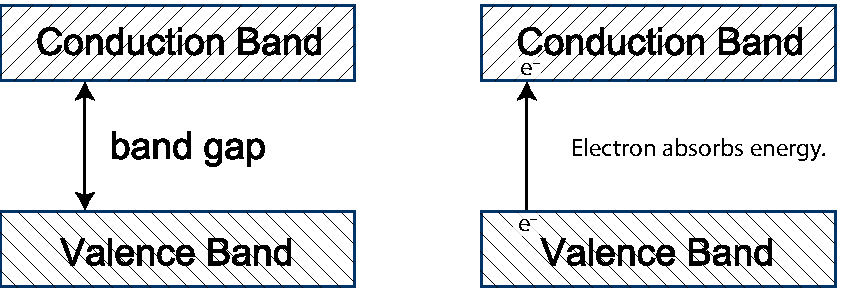
\includegraphics[width=.65\columnwidth]{energybands.pdf} 
\caption{(left) The band model approximates the discrete energy states in the valence and conduction band as a continuum.  Electrons in the valence band cannot conduct current as they are in covalent bonds.  Electrons in the conduction band can respond to external fields and result in net current flow.  (right)  Electrons in the valence band can gain energy from photons or phonons (lattice vibrations) and move into the conduction band.  The phonon or photon must have sufficient energy to cross the \emph{band gap}, which is a forbidden state.}
\label{fig:slide24b}
\end{figure}

As discussed previously, thermal energy is very low on average ($\sim 25$meV), but there are a few (very few) high energy electrons.   So the conductivity of semiconductors is poor, but not zero.  As shown in Fig.~\ref{fig:slide24b}, electrons in the valence band can gain energy from incoming photons or from the vibration in the crystal (phonons) and if the energy is sufficiently large, they can absorb  it and go into the conduction band.
%%%%%%%%%%%%%%%%%%%%%%%%%%%%%%%%%%%%%%%%%%%%
%             SUBSECTION 3.3.5             %
%%%%%%%%%%%%%%%%%%%%%%%%%%%%%%%%%%%%%%%%%%%%
\subsection{Model for Good Conductor}
 Given this background, we can now model a good conductor as a collection of atoms that are all ionized forming a  “sea” of electrons can wander about crystal, shown in Fig.~\ref{fig:slide25}.   The electrons are the “glue” that holds the solid together.  They spend most of their time in between the ionized nuclei, effectively shielding the nuclei from each other, lowering the energy of the system.  But they are not confined to bonds, they are free to move around the crystal and contribute to conduction.  Since they are “free”, they respond to applied fields and give rise to ohmic currents.  They also respond to incoming photons and give rise to the optical properties such as the fact that these materials are opaque and have shiny surfaces.   Electrons at the surface of the structure readily accept optical photons and re-radiate them.
%%%%%%%%%%%%%%%%%%%%%%%%%%%%%%%%%%%%%%%%%%%%
%                 FIGURE                   %
%%%%%%%%%%%%%%%%%%%%%%%%%%%%%%%%%%%%%%%%%%%%
\begin{figure}
\centering
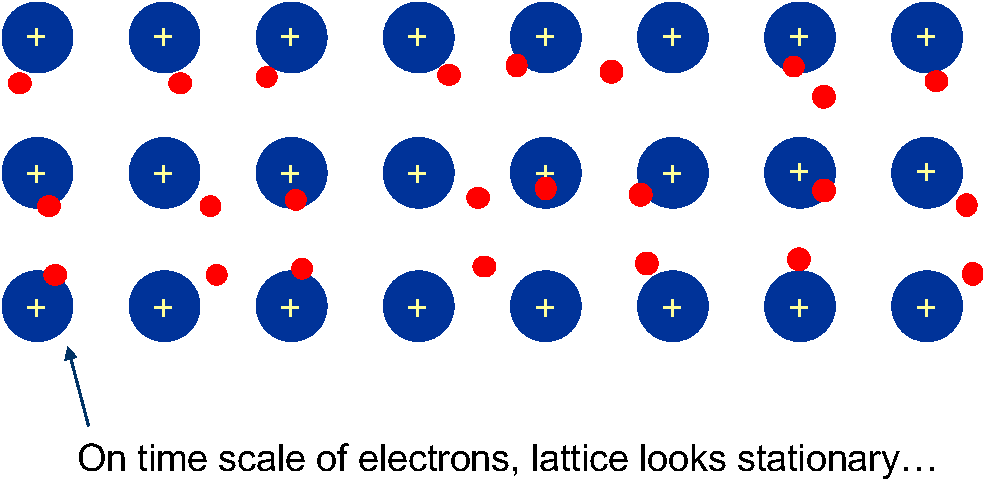
\includegraphics[width=.6\columnwidth]{slide25}
\caption{Model for good conductor has many ionized atoms arranged in a crystal surrounded by clouds of free electrons that "glue" the atoms together.}
\label{fig:slide25}
\end{figure}
%%%%%%%%%%%%%%%%%%%%%%%%%%%%%%%%%%%%%%%%%%%%
%              SUB-SUBSECTION              %
%%%%%%%%%%%%%%%%%%%%%%%%%%%%%%%%%%%%%%%%%%%%
\subsubsection{Semiconductor Bond Model}
Unlike a conductor, a semiconductor does not have many free electrons.  This is because all of the electrons are forming bonds in the crystal.  How can we free electrons ?  Either by giving them enough energy to break free (photons or very high energy phonons) or we have to introduce impurities in the crystal structure that have a different number of bonding electrons.  We'll discuss this in details next.
%%%%%%%%%%%%%%%%%%%%%%%%%%%%%%%%%%%%%%%%%%%%
%             SUBSECTION 3.3.6             %
%%%%%%%%%%%%%%%%%%%%%%%%%%%%%%%%%%%%%%%%%%%%
\subsection{Bond Model for Silicon (\texorpdfstring{$T=0\;K$}{T=0K})}
Let's build a simple 2D model for silicon as shown in Fig.~\ref{fig:silicon_model}.  The circles represent the nuclei and the lines represent electrons that are forming covalent bonds, or residing in the 3(sp)$^4$ orbitals.  For simplicity, we squashed the orbitals to lie on a plane.
%%%%%%%%%%%%%%%%%%%%%%%%%%%%%%%%%%%%%%%%%%%%
%                 FIGURE                   %
%%%%%%%%%%%%%%%%%%%%%%%%%%%%%%%%%%%%%%%%%%%%
\begin{figure}[tb]
\centering
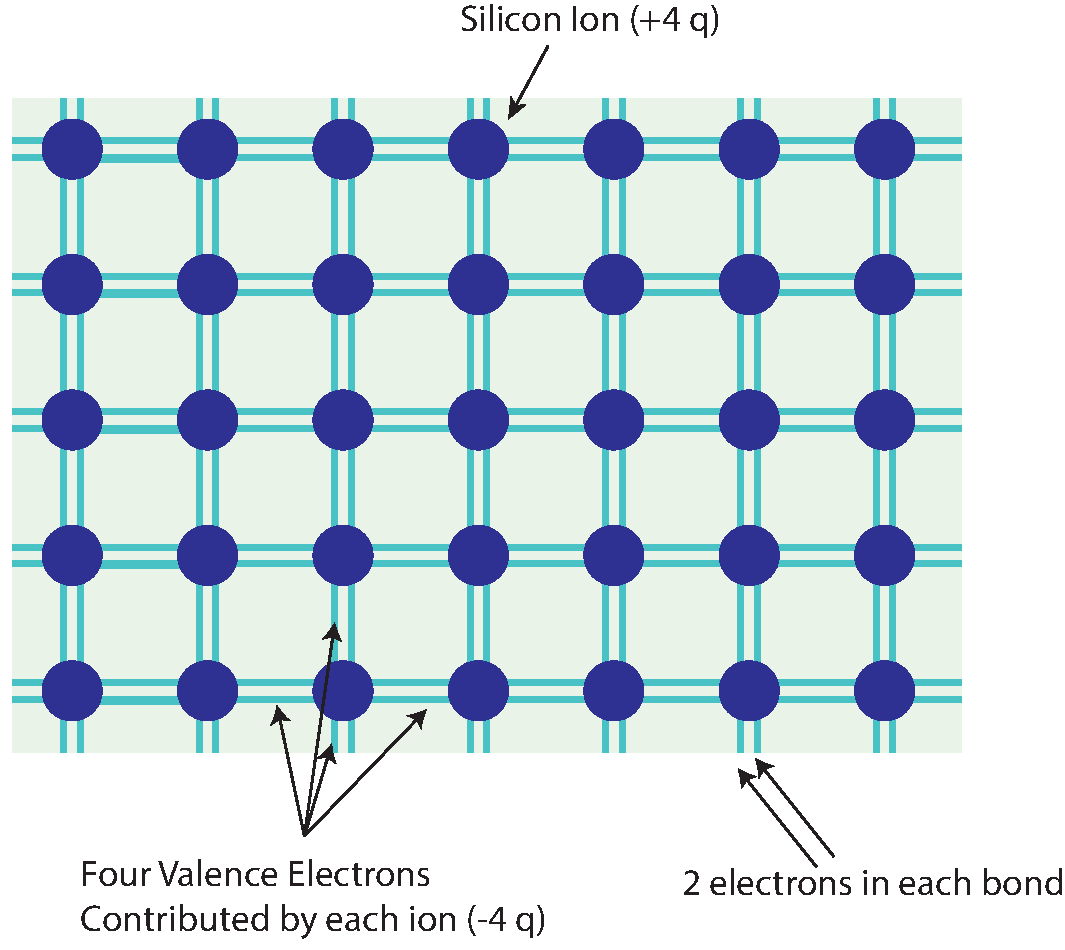
\includegraphics[width=.65\columnwidth]{silicon_model}
\caption{Simplified model for the  silicon crystal at $T=0^\circ$K.}
\label{fig:silicon_model}
\end{figure}

Each bond holds two electrons with opposite spin.  Each atom contributes 4 valence electrons to the orbital and borrows 4 electrons from 4 neighbors.  Thus each atom experiences a lower energy state corresponding to having a full orbital, despite being a group 4 element.  All the electrons are busy orbiting the nuclei and none can contribute to current conduction.
%%%%%%%%%%%%%%%%%%%%%%%%%%%%%%%%%%%%%%%%%%%%
%             SUBSECTION 3.3.7             %
%%%%%%%%%%%%%%%%%%%%%%%%%%%%%%%%%%%%%%%%%%%%
\subsection{Bond Model for Silicon (\texorpdfstring{$T>0\;K$}{T > 0K})}
%%%%%%%%%%%%%%%%%%%%%%%%%%%%%%%%%%%%%%%%%%%%
%                 FIGURE                   %
%%%%%%%%%%%%%%%%%%%%%%%%%%%%%%%%%%%%%%%%%%%%
\begin{figure}[tb]
\centering
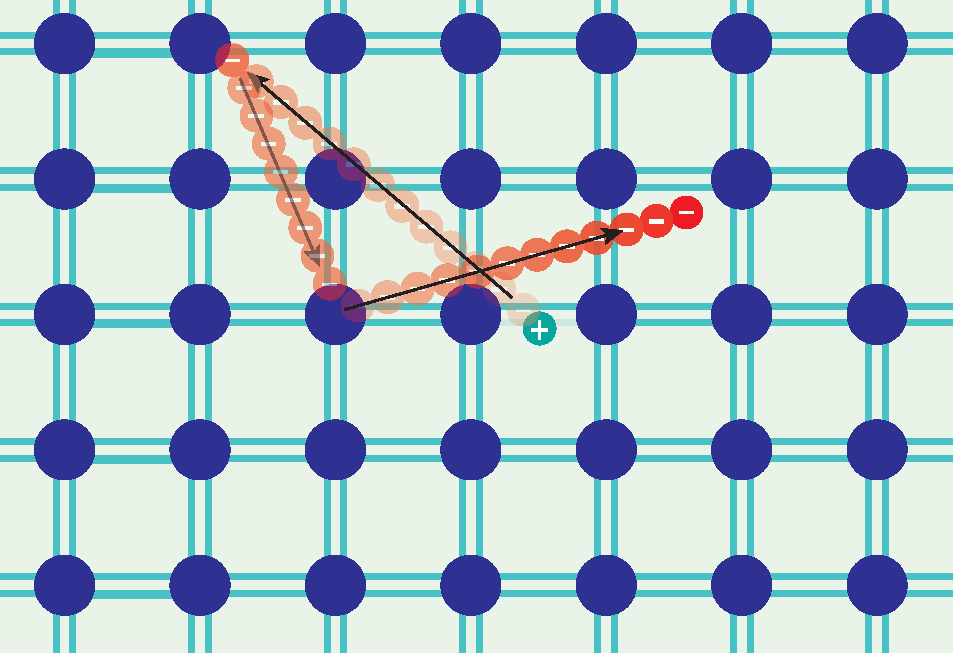
\includegraphics[width=.5\columnwidth]{silicon_broken_bond_motion}
\caption{In the silicon crystal, when a bond is broken, we create both a free electron and and a free hole.  The hole is a fictitious particle that behaves like a real particle in every way. It represents the motion of many electrons in the valence band.}
\label{fig:silicon_broken_bond}
\end{figure}

Now let's suppose we increase the temperature, which means the crystal lattice can absorb energy in the form of vibrations.  \footnote{Quantum mechanically, these vibrations can be treated as particle "phonons" (in analogy with photons) which can exchange energy with the electrons.}  Occasionally enough energy can be absorbed by a valence electron to be broken free from the lattice structure.  In the energy band model, we know the energy absorbed has to be at least as large as the band gap.  Once an electron becomes a conduction band electron, it's free to roam the crystal like a free electron.  The mass of the electron is not the same as the mass of an electron in a pure vacuum.  That's because the electron will still feel the influence of the crystal potential, which varies periodically.  It turns out that we can define an "effective" mass for the electron and treat it as if it were free and in vacuum, free from the influence of the crystal potential. 
%%%%%%%%%%%%%%%%%%%%%%%%%%%%%%%%%%%%%%%%%%%%
%             SUBSECTION 3.3.8             %
%%%%%%%%%%%%%%%%%%%%%%%%%%%%%%%%%%%%%%%%%%%%
\subsection{Holes?}
When we formed a free electron, we leave behind a broken bond.  This bond means the host atom has net charge.  But this charge corresponding to the vacancy is "fixed", right?
%%%%%%%%%%%%%%%%%%%%%%%%%%%%%%%%%%%%%%%%%%%%
%                 FIGURE                   %
%%%%%%%%%%%%%%%%%%%%%%%%%%%%%%%%%%%%%%%%%%%%
\begin{figure}[tb]
\centering
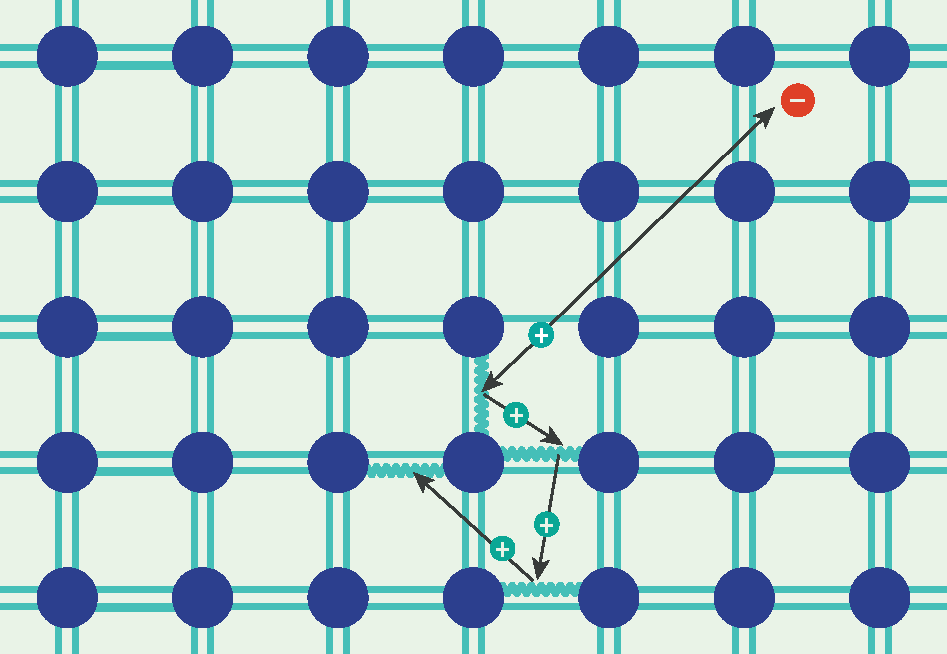
\includegraphics[width=.5\columnwidth]{silicon_hole}
\caption{Illustration of how a broken covalent bond moves around the crystal like a free particle.   Each wiggly bond represents a valence band electron moving into the vacancy created by the hole.} \label{fig:silicon_hole}
\end{figure}

Notice, as illustrated in Fig.~\ref{fig:silicon_hole},  that the vacancy (hole) left behind can be filled by a neighboring electron.   But if the neighboring electron jumps into this vacancy, it forms its own vacancy while filling the other one.  This chain reaction of vacancies moving around is complex as it corresponds to the motion of many valence band electrons.  An easy way to model it is to great it like there is a positive charge traveling around.  We call this positive (ficticious\footnote{Calling it real or fake is almost a philosophical question.  If it looks like a duck, swims like a duck, and quacks like a duck, then it probably is a duck.} ) particle a "hole".  It turns out that we can treat the holes as legitimate particles with positive mass and of course positive charge (because the broken bond leaves behind a net charge of +1).
%%%%%%%%%%%%%%%%%%%%%%%%%%%%%%%%%%%%%%%%%%%%
%             SUBSECTION 3.3.9             %
%%%%%%%%%%%%%%%%%%%%%%%%%%%%%%%%%%%%%%%%%%%%
\subsection{Yes, Holes!}
Using results from solid state theory, it can be shown that the net motion of many electrons in the valence band can be equivalently represented as the motion of a hole.  The picture is more complicated because electrons near the valence band edge have negative effective mass !  This is why the hole model is works as it does, something we’re not going to worry about in this chapter (or book).  Another common analog is to say a hole is like a bubble in a bottle. It can move around as if it were a free particle, but in fact its motion is the result of the motion of a lot of water molecules.  If we completely fill the bottle up, there’s no opportunity for a bubble to float around.  In the same way, a filled valence band does not contribute current.  Even if the electrons are moving (due to motion in the bond), the net current is zero
\begin{equation}
	\sum\limits_{Filled\,Band} {( - q){v_i}} = 0
\end{equation}
Now let’s take a partially filled band and play a trick.  Let’s say a partially filled band is a full band minus some electrons that we need to take out of the valence band to make it full: 
\begin{equation}
{J_{vb}} = \sum\limits_{vb} {( - q){v_i}}  = \sum\limits_{Filled\,Band} {( - q){v_i} - \sum\limits_{Empty\,States} {( - q){v_i}} }
\end{equation}
Since the first term is the full band and it does not contribute any current, the resulting current is due to the electrons we subtracted out to make a partially filled band.  In other words, the current is due to the empty states and even though the charges are negative, they act like positive charges:
\begin{equation}
{J_{vb}} =  - \sum\limits_{Empty\,States} {( - q){v_i}}  = \sum\limits_{Empty\,States} {q{v_i}}
\end{equation}
%%%%%%%%%%%%%%%%%%%%%%%%%%%%%%%%%%%%%%%%%%%%
%             SUBSECTION 3.3.10            %
%%%%%%%%%%%%%%%%%%%%%%%%%%%%%%%%%%%%%%%%%%%%
\subsection{More About Holes}
When a conduction band electron encounters a hole, the process is called \textit{recombination}.  The electron can fill the void, so we say that the electron and hole annihilate one another thus depleting the supply of free carriers.  This happens by chance as free electrons roam about and encounter holes.  So this recombination process depletes the crystal of both free electrons and free holes.  In thermal equilibrium it stands to reason that there must be a generation process to counterbalances to produce a steady stream of carriers.  This is of course the thermal generation we considered before.
%%%%%%%%%%%%%%%%%%%%%%%%%%%%%%%%%%%%%%%%%%%%%%%%%%%%%%%%%%%%%%%%%%%%%%%%%%%%%%%%%%%%%%%%
%%%%%%%%%%%%%%%%%%%%%%%%%%%%%%%%%%%%%%%%%%%%%%%%%%%%%%%%%%%%%%%%%%%%%%%%%%%%%%%%%%%%%%%%
%                                   SECTION 3.4                                        %
%%%%%%%%%%%%%%%%%%%%%%%%%%%%%%%%%%%%%%%%%%%%%%%%%%%%%%%%%%%%%%%%%%%%%%%%%%%%%%%%%%%%%%%%
%%%%%%%%%%%%%%%%%%%%%%%%%%%%%%%%%%%%%%%%%%%%%%%%%%%%%%%%%%%%%%%%%%%%%%%%%%%%%%%%%%%%%%%%
\section{Intrinsic Carrier Concentration}
%%%%%%%%%%%%%%%%%%%%%%%%%%%%%%%%%%%%%%%%%%%%
%             SUBSECTION 3.4.1             %
%%%%%%%%%%%%%%%%%%%%%%%%%%%%%%%%%%%%%%%%%%%%
\subsection{Thermal Equilibrium (Pure Si)}
In thermal equilibrium, there must be a balance between generation and recombination, otherwise a material would have more and more carriers spontaneously over time due to generation.  To determine the thermal equilibrium concentration of holes, $p_0$, and electrons $n_0$, first observe that  every time we create a free electron, we also create a free hole.  Likewise, every time a hole and electron recombine,both the free hole and free electron carrier concentration drop together.  So that means that $n_0 =  p_0 $.

Since the generation process is thermal in nature, we expect that the generation rate to be a strong function of temperature.

Let’s say $G$ represents the total about of free carrier generation per unit of time, or the rate of carrier generation:
\begin{equation} G = {G_{th}}(T) + {G_{opt}} \end{equation}
Note that in general we include thermal and optical carrier generation.  For the sake of simplicity, we’ll ignore the optical generation.  Now what about the recombination rate ?  You might expect the rate to be proportional to the concentration of electrons and holes as follows:
\begin{equation} R = k(n \times p) \end{equation}
Simply stated, the chance that an electron and a hole will meet and annihilate should depend on how many free electrons and or holes there are, with some proportionality constant $k$ that might be quite complicated.  In other words, the more carriers we have around, it’s logical to assume the rate will increase. 

Getting back to thermal equilibrium, if we assume the rate of generation and recombination are balanced, we can say
\begin{equation} G = R \end{equation}
Substituting for the recombination rate
\begin{equation} k(n \times p) = {G_{th}}(T) \end{equation}
The right hand side is a function of temperature.  We are not concerned with the details of how it varies for now, but we can say it’s a constant for a fixed $T$.  We call it $n_i^2$ because it has the units of concentration of carriers squared:
\begin{equation} n \times p = {G_{th}}(T)/k = {n_i}^2(T) \end{equation}
Since $n=p$ for an intrinsic (undoped) silicon crystal, we call it the \emph{intrinsic carrier concentration} $n_i$.  One can calculate the value of $n_i$ using techniques from solid-state physics and the value is approximately given by 
\begin{equation} {n_i}(T) \cong {10^{10}}{\rm{c}}{{\rm{m}}^{ - 3}}\,{\rm{at}}\,300\,{\rm{K}}
\end{equation}
We call this the Law of Mass-Action:
\begin{equation}
        p \cdot n = n_i^2
\end{equation}
%%%%%%%%%%%%%%%%%%%%%%%%%%%%%%%%%%%%%%%%%%%%
%             SUBSECTION 3.4.2             %
%%%%%%%%%%%%%%%%%%%%%%%%%%%%%%%%%%%%%%%%%%%%
\subsection{Generation Statistics}
 The rate at which carriers are generated is a strong function of the material bandgap $E_g$ (the distance between the valence band and conduction band), because it takes that much energy to promote an electron (or that much energy to break the bond).  Since the mechanism for is \textit{thermal} (vibrations), the hotter the temperature, the more generation.    It can be shown that the rate of generation is given by the following equation (approximately):
\begin{equation}
        n_i \propto e^{-E_g/2kT}
\end{equation}
Recall that $kT$ is proportional to the thermal energy and  $E_g$ is the band gap.  The above equation says that the number of carriers at an “excess” energy above the valence band depends strongly on how much thermal energy we have in the system.  The origin of this equation can be explained using a simple analogy.  Instead of a band gap, imagine a wall.  Let’s say that the wall is 6.5 feet tall and anyone with a height over 5.8 feet can hop over the wall.  If we take a classroom full of students and plot the distribution of heights, we get a normal distribution as shown in Fig.~\ref{fig:normal_dist}.  The average height is 5.3 feet and we have marked the local of 5.8, the necessary energy required to get over this wall.  If we integrate under the curve to find the total number of students tall enough, we can see that it’s not unreasonable that the integral over the tail of the distribution is approximately exponential as we have claimed.  If we raise the barrier height, exponentially fewer students can make it over the wall.
%%%%%%%%%%%%%%%%%%%%%%%%%%%%%%%%%%%%%%%%%%%%%%%%%%%%%%%%%%%%%%%%%%%%%%%%%%%%%%%%%%%%%%%%
%%%%%%%%%%%%%%%%%%%%%%%%%%%%%%%%%%%%%%%%%%%%%%%%%%%%%%%%%%%%%%%%%%%%%%%%%%%%%%%%%%%%%%%%
%                                   SECTION 3.5                                        %
%%%%%%%%%%%%%%%%%%%%%%%%%%%%%%%%%%%%%%%%%%%%%%%%%%%%%%%%%%%%%%%%%%%%%%%%%%%%%%%%%%%%%%%%
%%%%%%%%%%%%%%%%%%%%%%%%%%%%%%%%%%%%%%%%%%%%%%%%%%%%%%%%%%%%%%%%%%%%%%%%%%%%%%%%%%%%%%%%
\section{Doping with Impurities}
The term doping means that we add impurities to the crystal to change its properties.  As we’ll show, the presence of impurities can have a profound impact on the properties of a semiconductor.
%%%%%%%%%%%%%%%%%%%%%%%%%%%%%%%%%%%%%%%%%%%%
%             SUBSECTION 3.5.1             %
%%%%%%%%%%%%%%%%%%%%%%%%%%%%%%%%%%%%%%%%%%%%
\subsection{Doping with Group V Elements}
Let’s start with a group V element on the periodic table, for example Phosphorous (P) or Arsenic (As).  Because these are group 5 elements, they do not fit naturally in the crystal, that is unless they get rid of one of their valence electrons.  Then they can “fit in” and present to be silicon (group 4) atoms and form covalent bonds with their neighbors.  We are assuming that the number of group 5 elements is substantially smaller than the number of group 4 elements, so they would be more or less always surrounded by silicon atoms.  In our bonding model, we can say that the group 5 element fits into the crystal as an ionized atom by \emph{donating} an electron to the crystal, as shown in Fig.~\ref{fig:silicon_dopant_V}.   We call these dopants \emph{donors}.
%%%%%%%%%%%%%%%%%%%%%%%%%%%%%%%%%%%%%%%%%%%%
%                 FIGURE                   %
%%%%%%%%%%%%%%%%%%%%%%%%%%%%%%%%%%%%%%%%%%%%
\begin{figure}[tb]
\centering
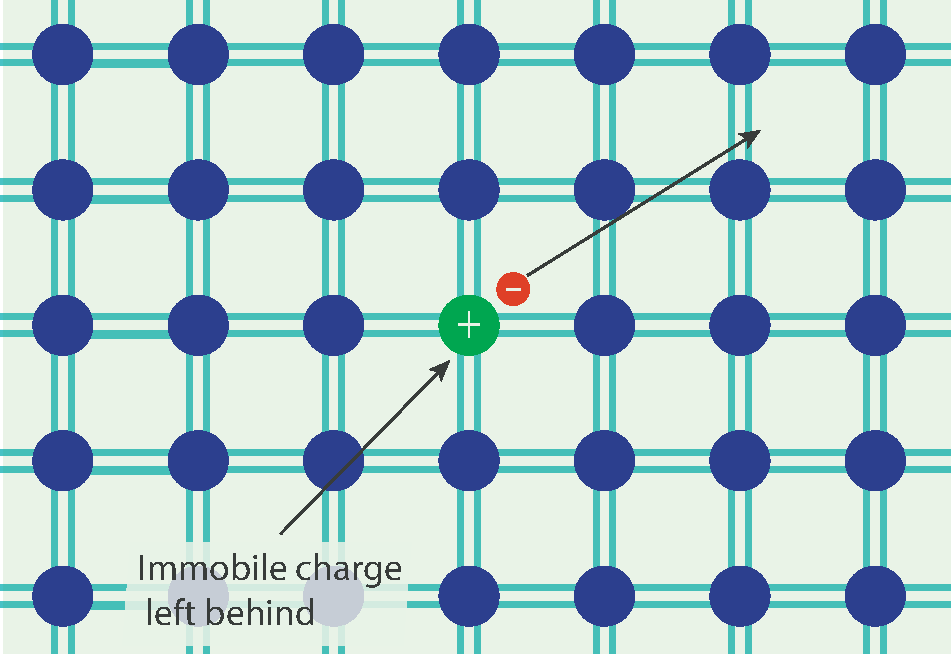
\includegraphics[width=.5\columnwidth]{silicon_dopant_V}
\caption{When a group V dopant (\emph{donor}) is added to the silicon crystal, it readily gives up one electron in order to form a covalent bond with its neighbors.  The extra electron is released and becomes a free carrier.}
\label{fig:silicon_dopant_V}
\end{figure}
%%%%%%%%%%%%%%%%%%%%%%%%%%%%%%%%%%%%%%%%%%%%
%             SUBSECTION 3.5.2             %
%%%%%%%%%%%%%%%%%%%%%%%%%%%%%%%%%%%%%%%%%%%%
\subsection{Donor Accounting}
Each ionized donor will contribute an extra “free” electron.  The material is charge neutral, so the total charge concentration must sum to zero:
\begin{equation}
        \rho  =  \underbrace{- q{n_0}}_{\text{free electrons}}
        + \underbrace{q{p_0}}_{\text{free holes}} +
        \underbrace{q{N_d}}_{\text{ions (immobile)}}  = 0
\end{equation}
By the Mass-Action Law:  $n \times p = {n_i}^2(T)$
\begin{equation}
         - q{n_0} + q\frac{{n_i^2}}{{{n_0}}} + q{N_d} = 0
\end{equation}
This leaves us with an equation involving only the density of free electrons:
\begin{equation}
- qn_0^2 + qn_i^2 + q{N_d}{n_0} = 0
\end{equation}
When we solve the quadratic pretty quickly since it’s quadratic:
\begin{equation}
n_0^2 - {N_d}{n_0} - n_i^2 = 0
\end{equation}
The general solution is given by
\begin{equation}
        {n_0} = \frac{{{N_d} \pm \sqrt {N_d^2 + 4n_i^2} }}{2}
\end{equation}
Only positive root is physically valid because it implies that the number of free electrons is larger than $N_d$.  Recall that we know there were $n_i$ free electrons before the dopants, and then we introduced the dopants and every dopant donates a free electron.  So why isn’t the free electron concentration simply $N_d + n_i$?  Because now the rate of recombination is higher and that’s exactly what the solution to the quadratic is telling us.  So clearly, only the positive root is physically valid and we have
\begin{equation}
        {n_0} = \frac{{{N_d} + \sqrt {N_d^2 + 4n_i^2} }}{2}
\end{equation}
For most practical situations:  ${N_d} \gg {n_i}$.  This means that we can simplify the quadratic to 
\begin{equation}
{n_0} = \frac{{{N_d} + {N_d}\sqrt {1 + 4{{\left( {\frac{{{n_i}}}{N}} \right)}^2}} }}{2} \approx \frac{{{N_d}}}{2} + \frac{{{N_d}}}{2} = {N_d}
\end{equation}
The final result is so obvious you might wonder why we bothered with all the questions.  It’s true, if you assume the doping concentration is very high, then the thermally generated electrons don’t matter and we can just assume that the number of free electrons is the same as the number of dopants.
%%%%%%%%%%%%%%%%%%%%%%%%%%%%%%%%%%%%%%%%%%%%
%             SUBSECTION 3.5.3             %
%%%%%%%%%%%%%%%%%%%%%%%%%%%%%%%%%%%%%%%%%%%%
\subsection{Doping with Group III Elements}
So we have seen that adding a group 5 element doping element increases the number of free electrons.  How about if we want to increase the number of holes?  Well, by symmetry, let’s try a group 3 element.  Boron for example has 3 bonding electrons, and so if it were surrounded by group 4 elements like silicon, it would be sorely missing an electron.  What can happen is that another electron can come to the rescue and make Boron a very happy atom. It’ll be a negatively charged ion (because it has an extra electron attached to it), but it can now covalently bond with its neighbors in an orderly fashion.  But where does that electron come from?  A neighboring atom for example can lose its electron, forming a hole, and that hole can now roam about as a free hole.  The model is illustrated in Fig.~\ref{fig:silicon_dopant_III}, and shows that the addition of a group 3 element creates a negatively charged ion and a free hole.
%%%%%%%%%%%%%%%%%%%%%%%%%%%%%%%%%%%%%%%%%%%%
%                 FIGURE                   %
%%%%%%%%%%%%%%%%%%%%%%%%%%%%%%%%%%%%%%%%%%%%
\begin{figure}[tb]
\centering
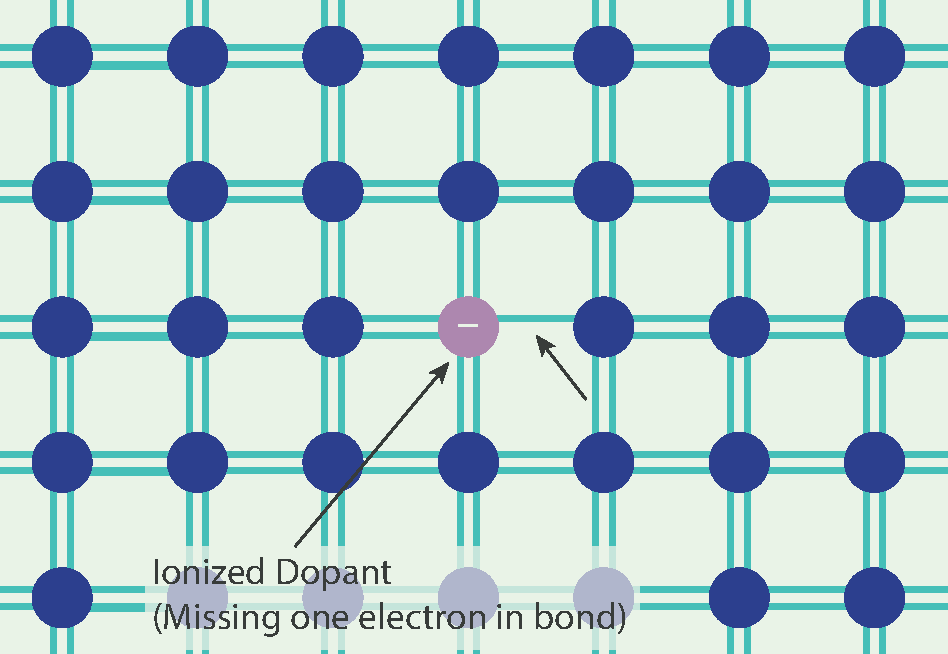
\includegraphics[width=.5\columnwidth]{silicon_dopant_III}
\caption{When a group III dopant (\emph{acceptor}) is added to the silicon crystal, it needs an electron to form a covalent bond with its neighbors, which it readily accepts from a nearby bond.  This electron, coming from another bond, creates a free hole.}
\label{fig:silicon_dopant_III}
\end{figure}

We don’t need to repeat the math, we can just note the final result of the group 5 case and just note that if the doping concentration is much larger than $n_i$, then the number of free holes will simply equal to the number of ionized dopants, which at normal room temperature is more or less all of them.\footnote{Freeze out is a condition you may encounter if you cool a semiconductor.  In this scenario, there isn’t enough energy to ionize the dopants, and the results of this section are no longer valid.}. We call group III dopants as “acceptors” because they accept an electron to form a covalent bond as opposed to group V dopants, which “donate” an electron and are known as “donors” as we noted above.
%%%%%%%%%%%%%%%%%%%%%%%%%%%%%%%%%%%%%%%%%%%%
%             SUBSECTION 3.5.4             %
%%%%%%%%%%%%%%%%%%%%%%%%%%%%%%%%%%%%%%%%%%%%
\subsection{Mass Action-Law (Again)}
The balance between generation and recombination means that in any given scenario, the product of the concentration of holes and electrons is constant.  
\begin{equation}
        {p_o} \cdot {n_o} = {n_i}^2
\end{equation} 
When a process creates holes and electrons asymmetrically, as we have just seen with dopants, then these extra free carriers will drive down the number of free carriers of opposite type due to recombination.   Recall that at $(T = 300\,{\rm{K}},\,\,{n_i} = {10^{10}}{\rm{c}}{{\rm{m}}^{ - 3}})$.  Now for the N-type doping case, the concentration of electronics is approximately equal to the number of ionized dopants $N_d^+$, or approximately equal to the number of dopants:
\begin{equation}
{n_0} = N_d^+  \cong {N_d}
\end{equation}
And that means that the number of holes has been reduced due to the increased presence of electrons:
\begin{equation}
        p_0 = \frac{n_i^2}{N_d}
\end{equation}
The same is true for a P-type scenario:
\begin{equation}
{p_0} = N_a^ -  \cong {N_a} 
\end{equation}
These extra holes drive down the concentration of electrons 
{ P-type case:} \begin{equation}
        n_0 = \frac{n_i^2}{N_a}
\end{equation}
%%%%%%%%%%%%%%%%%%%%%%%%%%%%%%%%%%%%%%%%%%%%
%             SUBSECTION 3.5.5             %
%%%%%%%%%%%%%%%%%%%%%%%%%%%%%%%%%%%%%%%%%%%%
\subsection{Compensation}
What happens if we dope with \textit{both} donors and acceptors?  Who wins out ?  Well, it depends on the doping level.  Essentially we create both free electrons for every donor dopant and free holes for every acceptor dopant.  Take a look at Fig.~\ref{fig:silicon_dopant_both}.
%%%%%%%%%%%%%%%%%%%%%%%%%%%%%%%%%%%%%%%%%%%%
%                 FIGURE                   %
%%%%%%%%%%%%%%%%%%%%%%%%%%%%%%%%%%%%%%%%%%%%
\begin{figure}[tb]
\centering
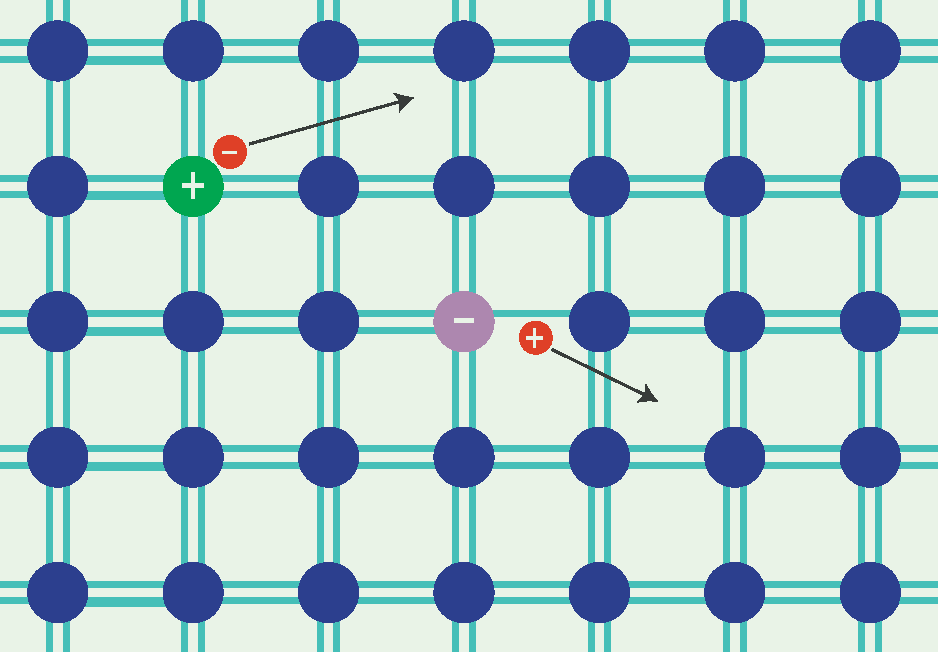
\includegraphics[width=.5\columnwidth]{silicon_dopant_both}
\caption{Silicon crystal doped by both an acceptor and donor dopant results in the creation of both free holes and electrons.}
\label{fig:silicon_dopant_both}
\end{figure}

If we dope with more donors than acceptors and $N_d > N_a$, then the material is “n-type” because the action of the free electrons is more than the free holes.  In other words, the free electron density is given by
\begin{equation}
        {n_o} = {N_d} - {N_a} \gg {n_i}
\end{equation}
And the free holes are approximately given by the law of Mass-Action:
\begin{equation}
        {p_o} = \frac{{n_{_i}^2}}{{{N_d} - {N_a}}}
\end{equation}
On the other hand, if we have more acceptors than donors, or  $N_a > N_d$, then we can approximate the number of free holes by
\begin{equation}
        {p_o} = {N_a} - {N_d} \gg {n_i}
\end{equation}
And the number of free electrons by
\begin{equation}
        {n_o} = \frac{{n_{_i}^2}}{{{N_a} - {N_d}}}
\end{equation}
%%%%%%%%%%%%%%%%%%%%%%%%%%%%%%%%%%%%%%%%%%%%%%%%%%%%%%%%%%%%%%%%%%%%%%%%%%%%%%%%%%%%%%%%
%%%%%%%%%%%%%%%%%%%%%%%%%%%%%%%%%%%%%%%%%%%%%%%%%%%%%%%%%%%%%%%%%%%%%%%%%%%%%%%%%%%%%%%%
%                                   SECTION 3.6                                        %
%%%%%%%%%%%%%%%%%%%%%%%%%%%%%%%%%%%%%%%%%%%%%%%%%%%%%%%%%%%%%%%%%%%%%%%%%%%%%%%%%%%%%%%%
%%%%%%%%%%%%%%%%%%%%%%%%%%%%%%%%%%%%%%%%%%%%%%%%%%%%%%%%%%%%%%%%%%%%%%%%%%%%%%%%%%%%%%%%
\section{Drift Currents}
Given what we have learned about a semiconductor, we can see that it has some resemblance to the ideal gas model we developed earlier.  In particular, we have some concentration of “free” carriers that roam the crystal with thermal energy and can respond to an external field.  
%%%%%%%%%%%%%%%%%%%%%%%%%%%%%%%%%%%%%%%%%%%%
%             SUBSECTION 3.6.1             %
%%%%%%%%%%%%%%%%%%%%%%%%%%%%%%%%%%%%%%%%%%%%
\subsection{Thermal Equilibrium}
The rapid, random motion of holes and electrons is quite fast because these particles are so light.  The “thermal velocity” is approximately $v_{th} = 10^7$ cm/s, and the number of collisions happens on a time scale of approximately $\tau_c = 10^{-13}$s.  The thermal velocity can be approximated by equating the thermal energy with the kinetic energy
\begin{equation}
    {\frac{1}{2}}m_n^*v_{th}^2 = {\frac{1}{2}}kT
\end{equation}
During this time, the average carrier moves a distance of $\lambda$
\begin{equation} \lambda  = {v_{th}}{\tau _c}\end{equation}
Which is approximately
\begin{equation}
        \lambda  = {10^7}{\rm{cm}}/s \times {10^{ - 13}}s = {10^{ - 6}}{\rm{cm}}
\end{equation}
%%%%%%%%%%%%%%%%%%%%%%%%%%%%%%%%%%%%%%%%%%%%
%                 FIGURE                   %
%%%%%%%%%%%%%%%%%%%%%%%%%%%%%%%%%%%%%%%%%%%%
\begin{figure}[tb]
\centering
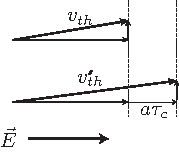
\includegraphics[width=.3\columnwidth]{drift_field}
\caption{The drift velocity will increase by the application of an electric field, on average by an amount $a \tau_c$, where $a$ is the acceleration from the field and $\tau_c$ is the time between collisions.}
\label{fig:drift_field}
\end{figure}
(hole case)
%%%%%%%%%%%%%%%%%%%%%%%%%%%%%%%%%%%%%%%%%%%%
%             SUBSECTION 3.6.2             %
%%%%%%%%%%%%%%%%%%%%%%%%%%%%%%%%%%%%%%%%%%%%
\subsection{Drift Velocity and Mobility}
Now, as before, we apply an electric field $E$ and charge carriers accelerate, at least for  $\tau_c$ seconds before they collide.
As shown in Fig.~\ref{fig:drift_field}, during this time they gain momentum from the field
\begin{equation}
        v_{dr} = a \tau_c = \frac{q E}{m} \tau_c
\end{equation}
Or in other words, the drift velocity is proportional to the field $E$
\begin{equation}
        v_{dr} = \frac{q \tau_c}{m} E = \mu_n E
\end{equation}
We define a mobility for both the electrons, $\mu_n$ and holes, $\mu_p$ and expect they will be different due to the difference in the effective mass between holes and electrons.
%%%%%%%%%%%%%%%%%%%%%%%%%%%%%%%%%%%%%%%%%%%%
%             SUBSECTION 3.6.3             %
%%%%%%%%%%%%%%%%%%%%%%%%%%%%%%%%%%%%%%%%%%%%
\subsection{Mobility vs. Doping in Silicon at \texorpdfstring{$300^\circ$}{300K}K}
%%%%%%%%%%%%%%%%%%%%%%%%%%%%%%%%%%%%%%%%%%%%
%                 FIGURE                   %
%%%%%%%%%%%%%%%%%%%%%%%%%%%%%%%%%%%%%%%%%%%%
\begin{figure}[tb]
\centering
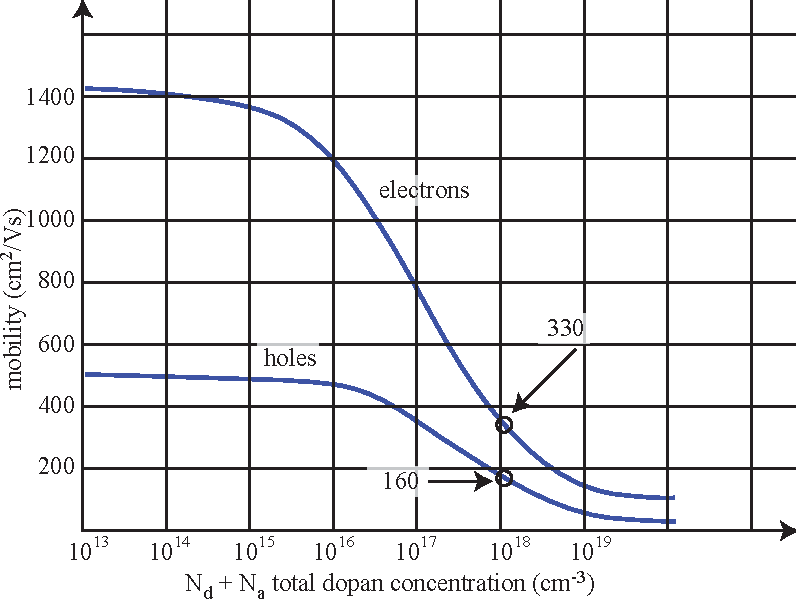
\includegraphics[width=.75\columnwidth]{mobility}
\caption{Mobility of electrons and holes in silicon as a function of \emph{total} doping concentration. }
\label{fig:mobility}
\end{figure}

As you might expect, the mobility should depend on temperature and also on the total dopant concentration, because the more dopants we introduce, the more scattering sites.  This is born out by measurement and theory, as shown in Fig.~\ref{fig:mobility}, which shows that the mobility is highest for undoped silicon and then begins to drop as we introduce more and more dopants.  A typical values for electrons is about ${\mu _n} = 1000 \mathrm{cm^2}/\mathrm{V s}$ and for holes ${\mu _p} = 400 \mathrm{cm^2}/\mathrm{V s}$.  Electrons go faster as they are “lighter”. 
%%%%%%%%%%%%%%%%%%%%%%%%%%%%%%%%%%%%%%%%%%%%%%%%%%%%%%%%%%%%%%%%%%%%%%%%%%%%%%%%%%%%%%%%
%%%%%%%%%%%%%%%%%%%%%%%%%%%%%%%%%%%%%%%%%%%%%%%%%%%%%%%%%%%%%%%%%%%%%%%%%%%%%%%%%%%%%%%%
%                                   SECTION 3.7                                        %
%%%%%%%%%%%%%%%%%%%%%%%%%%%%%%%%%%%%%%%%%%%%%%%%%%%%%%%%%%%%%%%%%%%%%%%%%%%%%%%%%%%%%%%%
%%%%%%%%%%%%%%%%%%%%%%%%%%%%%%%%%%%%%%%%%%%%%%%%%%%%%%%%%%%%%%%%%%%%%%%%%%%%%%%%%%%%%%%%
\section{Diffusion Currents}
We are all familiar with diffusion currents in everyday life, for example the fragrance of a bottle of perfume spreads across the room through the random motion of perfume molecules in air.   This motion is due to the fact that even through perfume molecules move randomly due to thermal energy, they move in directions from high concentration to low concentration.  Why does this happen exactly?
%%%%%%%%%%%%%%%%%%%%%%%%%%%%%%%%%%%%%%%%%%%%
%             SUBSECTION 3.7.1             %
%%%%%%%%%%%%%%%%%%%%%%%%%%%%%%%%%%%%%%%%%%%%
\subsection{Diffusion}
Let’s do a simple thought experiment to figure out why diffusion flows from high to low concentration.  In Fig.~\ref{fig:slide46}, imagine that we fill the left chamber with a gas at temperate $T$. If we suddenly remove the divider, what happens?  The gas will fill the entire volume of the new chamber. How does this occur?
%%%%%%%%%%%%%%%%%%%%%%%%%%%%%%%%%%%%%%%%%%%%
%                 FIGURE                   %
%%%%%%%%%%%%%%%%%%%%%%%%%%%%%%%%%%%%%%%%%%%%
\begin{figure}[tb]
\centering
\begin{tabular}{cc}
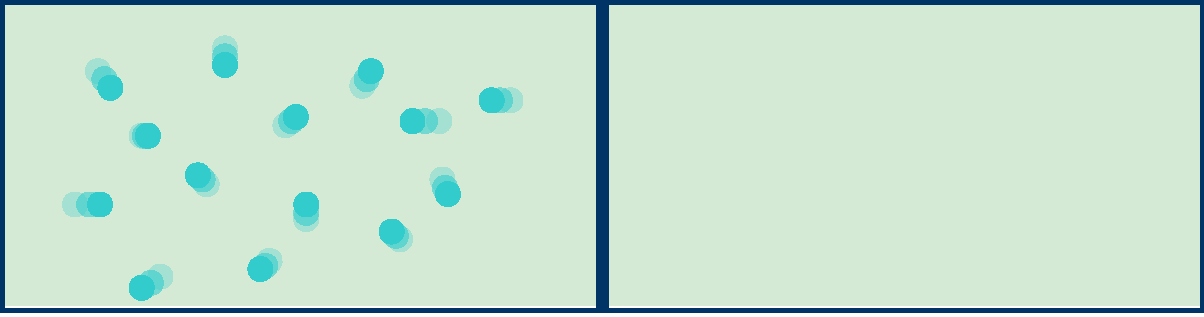
\includegraphics[width=.45\columnwidth]{partition_closed} &
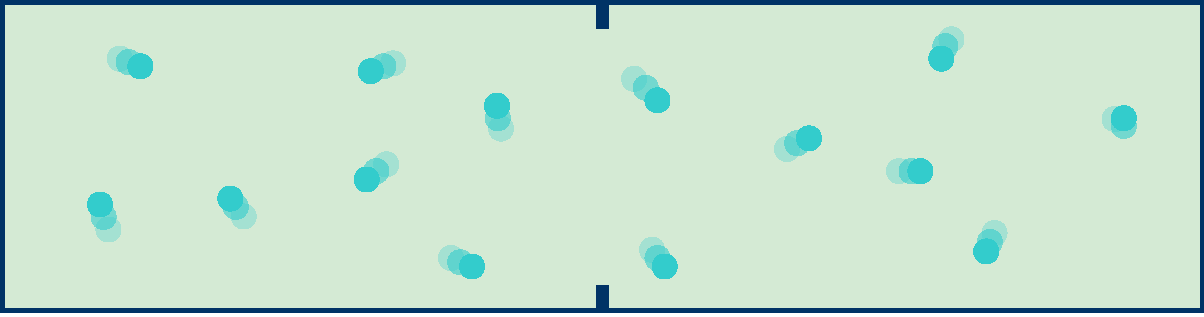
\includegraphics[width=.45\columnwidth]{partition_open}\\ 
 (a) & (b)\\
\end{tabular}
\caption{(a)  Particles moving randomly in a box with a partition are confined to the left partition.  (b)  When we open the partition, after a brief time we find particles distributed equally in both partitions.}
\label{fig:slide46}
\end{figure}
%%%%%%%%%%%%%%%%%%%%%%%%%%%%%%%%%%%%%%%%%%%%
%                 FIGURE                   %
%%%%%%%%%%%%%%%%%%%%%%%%%%%%%%%%%%%%%%%%%%%%
\begin{figure}[tb]
\centering
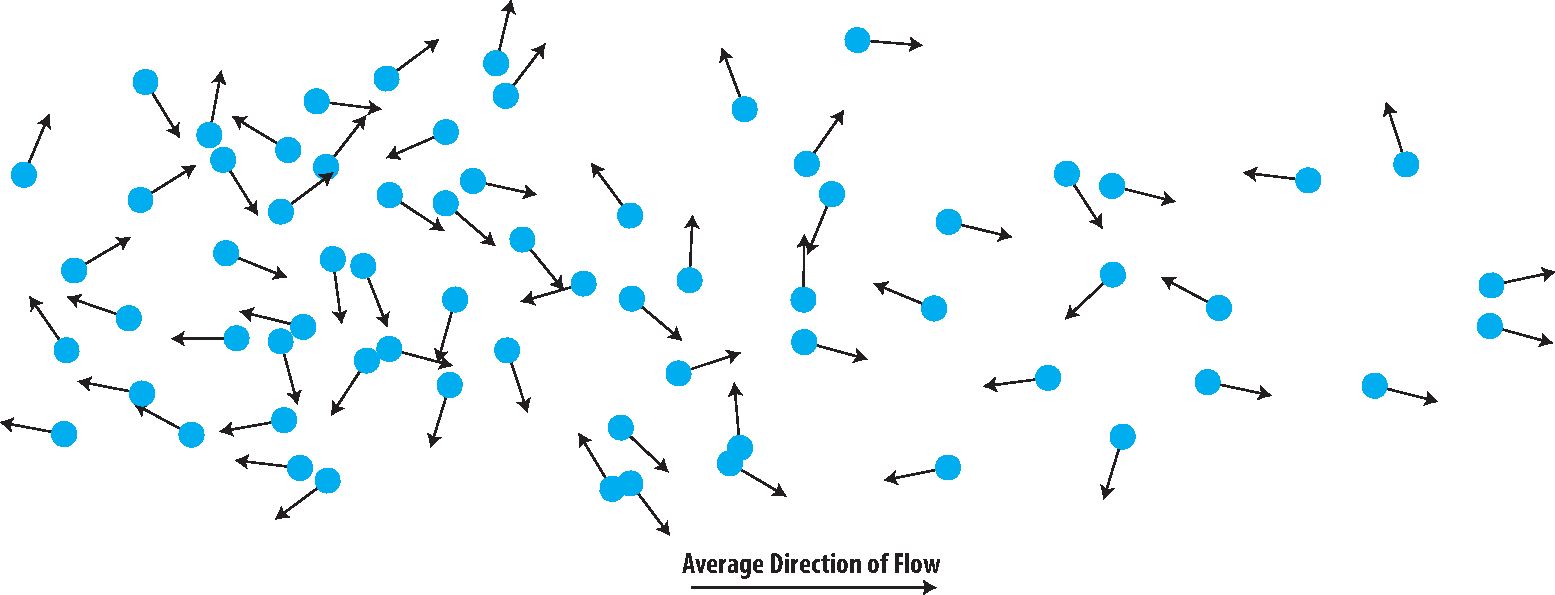
\includegraphics[width=.95\columnwidth]{random_flow}
\caption{Particles in random thermal motion move on average in every direction with equal probability.  If there's a concentration gradient, then regions of high concentration contribute more carriers moving towards regions of low concentration compared to particles from low concentrations, thus leading to diffusion.}
\label{fig:random_flow}
\end{figure}

Let’s zoom in to the motion of the molecules (Fig.~\ref{fig:random_flow}).  The net motion of gas molecules to the right chamber was due to the concentration gradient.
If each particle moves on average left or right with equal probability, then eventually half will be in the right chamber. If the molecules were charged (or electrons), then there would be a net current flow.  It's clear that the diffusion current flows from high concentration to low concentration, because in areas of higher concentration there are more particles moving both left and right, which is larger than say the particles moving left and righ in the regions of low concentration.
%%%%%%%%%%%%%%%%%%%%%%%%%%%%%%%%%%%%%%%%%%%%
%                 FIGURE                   %
%%%%%%%%%%%%%%%%%%%%%%%%%%%%%%%%%%%%%%%%%%%%
\begin{figure}[tb]
\centering
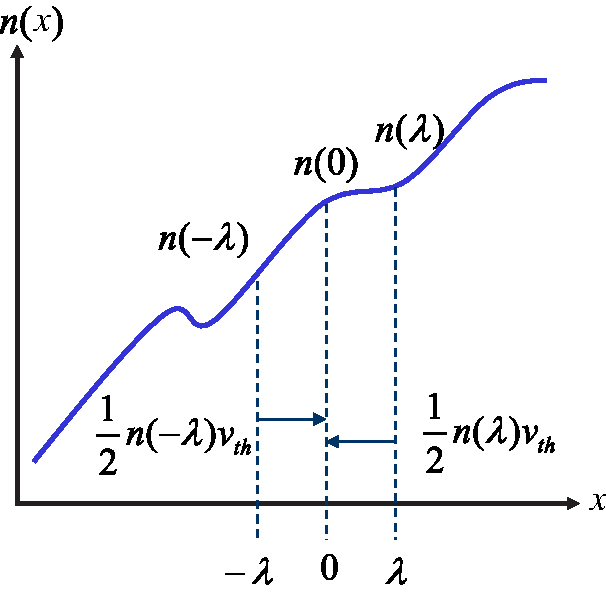
\includegraphics[width=.45\columnwidth]{slide48}
\caption{The distribution of electron concentration $n(x)$ leads to a diffusion current flow in the direction from high concentration to low concentration.  To show this, we consider how many particles cross a given point, $x=0$ for example, in a unit of time.  $\lambda$ is the average distance moved by particles in thermal motion.}
\label{fig:slide48}
\end{figure}
%%%%%%%%%%%%%%%%%%%%%%%%%%%%%%%%%%%%%%%%%%%%
%             SUBSECTION 3.7.2             %
%%%%%%%%%%%%%%%%%%%%%%%%%%%%%%%%%%%%%%%%%%%%
\subsection{Diffusion Equations}
We can find an equation for diffusion currents of electrons if we carefully consider the collective average motion.  With reference to Fig.~\ref{fig:slide48}, assume that the mean free path is $\lambda$.  Let’s find the flux of carriers crossing the $x=0$ plane by imagining how many particles will cross the origin in a time equal to the average inter-collision time.  If we move left and right a distance $\lambda$, then all particles moving in the right direction (towards the origin), will cross the origin as they travel on average a distance $\lambda$.  The flux of electrons is therefore the number of particles multiplied by the distance they move
\begin{equation}d
        F = \frac{1}{2}{v_{th}}\left( {n( - \lambda ) - n(\lambda )} \right)
\end{equation}
In the above equation, the factor $1/2$ arises because only half the particles from the left move right, and likewise half the particles on the right move left.  If the distance $\lambda$ is small, and $n$ is a smooth function, we can estimate the amount of carriers at each location by a simple Taylor series expansion
\begin{equation}
        F = \frac{1}{2}{v_{th}}\left( {\left[ {n(0) - \lambda \frac{{dn}}{{dx}}} \right] -
         \left[ {n(0) + \lambda \frac{{dn}}{{dx}}} \right]} \right)
\end{equation}
Which shows that it’s only the gradient of the concentration that contributes to current:
\begin{equation}
        F =  - {v_{th}}\lambda \frac{{dn}}{{dx}}
\end{equation}
Now, since electrons carry charge, the current flows in the opposite direction:
\begin{equation}
        J =  - qF = q{v_{th}}\lambda \frac{{dn}}{{dx}}
\end{equation}
%%%%%%%%%%%%%%%%%%%%%%%%%%%%%%%%%%%%%%%%%%%%
%             SUBSECTION 3.7.3             %
%%%%%%%%%%%%%%%%%%%%%%%%%%%%%%%%%%%%%%%%%%%%
\subsection{Einstein Relation}
The thermal velocity at a given temperature $T$ is given by
    \begin{equation}
        {\frac{1}{2}}m_n^*v_{th}^2 = {\frac{1}{2}}kT
    \end{equation}
And therefore the mean free path $lambda$ is given by
    \begin{equation}
        \lambda  = {v_{th}}{\tau _c}
    \end{equation}
The term we're interested in from the diffusion current equation is the product of $v_{th} \lambda$:
    \begin{equation}
        {v_{th}}\lambda  = v_{th}^2{\tau _c} = kT\frac{{{\tau _c}}}{{m_n^*}} = \frac{{kT}}{q}\frac{{q{\tau _c}}}{{m_n^*}}
    \end{equation}
which leads to
\begin{equation}
        J = q{v_{th}}\lambda \frac{{dn}}{{dx}} = q\left( {\frac{{kT}}{q}{\mu _n}} \right)\frac{{dn}}{{dx}}
\end{equation}
The term in the parenthesis is known as the Diffusion Constant, and it's related to the mobility: 
\begin{equation}
        {D_n} = \left( {\frac{{kT}}{q}} \right){\mu _n}
\end{equation}
%%%%%%%%%%%%%%%%%%%%%%%%%%%%%%%%%%%%%%%%%%%%
%             SUBSECTION 3.7.4             %
%%%%%%%%%%%%%%%%%%%%%%%%%%%%%%%%%%%%%%%%%%%%
\subsection{Total Current and Boundary Conditions}
When both drift and diffusion are present, the total current is given by the sum:
    \begin{equation}
        J = {J_{drift}} + {J_{diff}} = q{\mu _n}nE + q{D_n}\frac{{dn}}{{dx}}
    \end{equation}
In resistors, the carrier is approximately uniform and the second term is nearly zero. For currents flowing uniformly through an interface (no charge accumulation), as shown in Fig.~\ref{fig:slide50}, the field is discontinuous.  Nevertheless the current must flow through the interface (unless charge is accumulating):
    \begin{equation}
        {J_1} = {J_2}
    \end{equation}
This implies that:
    \begin{equation}
        {\sigma _1}{E_1} = {\sigma _2}{E_2}
    \end{equation}
So the electric field is discontinuous by the inverse ratio of conductivity:
    \begin{equation}
        \frac{{{E_1}}}{{{E_2}}} = \frac{{{\sigma _2}}}{{{\sigma _1}}}
    \end{equation}
%%%%%%%%%%%%%%%%%%%%%%%%%%%%%%%%%%%%%%%%%%%%
%                 FIGURE                   %
%%%%%%%%%%%%%%%%%%%%%%%%%%%%%%%%%%%%%%%%%%%%
\begin{figure}[tb]
\centering
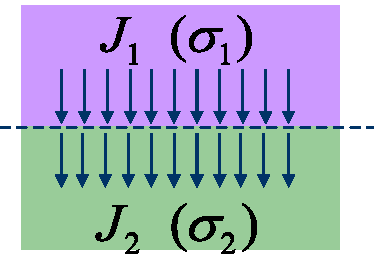
\includegraphics[width=.25\columnwidth]{slide50}
\caption{Uniform current flowing through a discontinuity in the conductivity must be accompanied by a discontinuity in the electric field.}
\label{fig:slide50}
\end{figure}
%%%%%%%%%%%%%%%%%%%%%%%%%%%%%%%%%%%%%%%%%%%%
%             SUBSECTION 3.7.5             %
%%%%%%%%%%%%%%%%%%%%%%%%%%%%%%%%%%%%%%%%%%%%
\subsection{Reference}
Edward Purcell, \textit{Electricity and Magnetism}, \textbf{Berkeley Physics Course Volume 2 (2nd Edition)}, pages 133-142.
